\begin{document}
\frontmatter
\title{Glimmer-CISM {\glimmerver} Documentation}
\author{Magnus Hagdorn\thanks{Magnus.Hagdorn@ed.ac.uk}, Ian
  Rutt\thanks{I.C.Rutt@bristol.ac.uk}, Tony Payne\thanks{A.J.Payne@bristol.ac.uk} 
  Felix Hebeler\thanks{fhebeler@geo.unizh.ch} and Timothy R. Wylie}
\maketitle
\tableofcontents

\ifthenelse{\boolean{html}}
{
\Configure{graphics*} 
         {eps} 
         {\Needs{"convert \csname Gin@base\endcsname.eps 
                               \csname Gin@base\endcsname.png"}% 
          \Picture[pict]{\csname Gin@base\endcsname.png}% 
         } 

}
{}

\mainmatter
\part{User Documentation}
\chapter{User Guide}
\newcommand{\dir}{ug}
This package provides an addon library to \href{http://developer.berlios.de/projects/glimmer-cism/}{Glimmer-CISM} which provides a bedrock erosion and sediment transport component. Drivers are provided for EISMINT type forcing and the EIS driver. You can use \texttt{erosion} with your own climate drivers (see Section \ref{erosion.sec.using_it}).

\section{Model Configuration}
Add a selection of the follwing configuration options to your GLIDE configuration file to enable and control erosion and sediment transport.
\begin{center}
  \tablefirsthead{%
    \hline
  }
  \tablehead{%
    \hline
    \multicolumn{2}{|l|}{\emph{\small continued from previous page}}\\
    \hline
  }
  \tabletail{%
    \hline
    \multicolumn{2}{|r|}{\emph{\small continued on next page}}\\
    \hline}
  \tablelasttail{\hline}
  \begin{supertabular*}{\textwidth}{@{\extracolsep{\fill}}|l|p{9cm}|}
    \hline
    \multicolumn{2}{|l|}{\texttt{[Erosion]}}\\
    \hline
    \multicolumn{2}{|p{0.95\textwidth}|}{Switch on hard bedrock erosion.}\\
    \hline
    \texttt{hb\_erosion} & set parameterisation of hard bedrock erosion\\
    \texttt{ntime} & update erosion calculation every \texttt{ntime} time steps\\
    \texttt{updeate\_topo} & whether erosion/sediment transport changes ice bed topography (default :1)\\
    \hline
    \hline
    \multicolumn{2}{|l|}{\texttt{[Basic\_Transport]}}\\
    \hline
    \multicolumn{2}{|p{0.95\textwidth}|}{Sediment transport is paramterised by assuming transport velocities are proportional to basal ice velocities (see Section \ref{erosion.sec.basic_trans})}\\
    \hline
    \texttt{deformable\_velo} & basal ice velocities are multiplied with this factor to get sediment transport velocities.\\
    \texttt{dirty\_ice\_thick} & thickness of dirty basal ice layer\\
    \texttt{soft\_a},  \texttt{soft\_b}& parameterisation of maximum deformable sediment layer thickness, $$z_{\text{max}}=a+b|\vec{\tau}_b|$$\\
    \hline
    \hline
    \multicolumn{2}{|l|}{\texttt{[Transport]}}\\
    \hline
    \multicolumn{2}{|p{0.95\textwidth}|}{Deforming sediment layer is based on some rheology (see Section \ref{erosion.sec.full_trans}).}\\
    \hline
    \texttt{dirty\_ice\_thick} & thickness of dirty basal ice layer\\
    \texttt{calc\_btrc} & sediment velocities set ice sliding velocities.\\
    \texttt{effective\_pressure} & set the effective pressure at the ice base.\\
    \texttt{pressure\_gradient} & set pressure gradient in sediment bed.\\
    \texttt{phi} & angle of internal friction, $\phi$.\\
    \texttt{cohesion} & cohesion of sediments.\\
    \texttt{a} & factor for sediment flow law.\\
    \texttt{m} & exponent of effective pressure.\\
    \texttt{n} & exponent of shear stress.\\
  \end{supertabular*}
\end{center}

\section{Using the Library}\label{erosion.sec.using_it}
The \texttt{erosion} module provides a number of subroutines which can be used to add erosion/sediment transport to an ice sheet model based on GLIMMER. Have a look at the EISMINT driver \texttt{simple\_erosion.f90}.

All variables associated with the module are stored in a derived type. Similarly to GLIDE you will need to declare a variable of that derived type:
\begin{verbatim}
type(erosion_type) :: er
\end{verbatim}
The erosion component is initialised after GLIDE was initialised using the call
\begin{verbatim}
call er_initialise(er,config,model)
\end{verbatim}
The erosion time step is done after the first GLIDE timestep:
\begin{verbatim}
call glide_tstep_p1(model,time)
call er_tstep(er,model)
\end{verbatim}
Finally, the model is shut down before GLIDE is shut down with
\begin{verbatim}
call er_finalise(er)
\end{verbatim}

%\section{Visualisation}\label{erosion.sec.vis_it}
%\texttt{erosion} comes with a number of python scripts for visualising sediments.
%
%\begin{pycf}{plot\_seds.py -T-1 -pprof --not\_p  fenscan.nc sediments.ps}{\dir/figs/sediments.eps}
%plots a map of sediment erosion/deposition of the last time slice. The \texttt{-p} option together with the \texttt{--not\_p} option plots the profile. This program plots sediment erosion/deposition relative to the initial sediment distribution. Blue areas indicate areas where sediments have been removed. Red areas indicate areas where sediments have been deposited.
%\end{pycf}
%
%\begin{pycf}{plot\_seds\_profile.py -t0. -e stages -pprof --not\_p fenscan.nc prof.ps}{\dir/figs/sed_profile.eps}
%plots a profile showing sediment erosion/deposition. A file containing timings of glacial stages is required. The time when sediments are deposited are indicated with colours found in this file. The \texttt{stages} file contains 4 comma--eparated columns. The first column contains the name, second and thrid column start and end time in years, and the last column a R/G/B triplet for the background colour.
%\end{pycf}


\chapter{Tutorial}
\renewcommand{\dir}{tut}
\newcommand{\dir}{tut}

\pagestyle{myheadings} \markright{GLIMMER {\glimmerver} --- Tutorial}

\begin{document}
\title{GLIMMER {\glimmerver} --- Tutorial}
\author{Felix Hebeler \thanks{fhebeler@geo.unizh.ch}}
\maketitle
\tableofcontents
\newpage

\newcommand{\dir}{tut}

\pagestyle{myheadings} \markright{GLIMMER {\glimmerver} --- Tutorial}

\begin{document}
\title{GLIMMER {\glimmerver} --- Tutorial}
\author{Felix Hebeler \thanks{fhebeler@geo.unizh.ch}}
\maketitle
\tableofcontents
\newpage

\newcommand{\dir}{tut}

\pagestyle{myheadings} \markright{GLIMMER {\glimmerver} --- Tutorial}

\begin{document}
\title{GLIMMER {\glimmerver} --- Tutorial}
\author{Felix Hebeler \thanks{fhebeler@geo.unizh.ch}}
\maketitle
\tableofcontents
\newpage

\input{\dir/tut.tex}
\end{document}

\end{document}

\end{document}


\part{Developer Documentation}

\chapter{Numerics}
\renewcommand{\dir}{num}
This part describes the numerical implementation of GLIMMER in some detail. It is hoped that more parts will be added in the future.
\section{Ice Thickness Evolution}
\label{sc:glide_thickness_evolution}
The evolution of the ice thickness, $H$, stems from the continuity equation and can be expressed as
\begin{equation}
  \label{kin.eq.ice_thickness}
  \frac{\pd H}{\pd t} = -\vec\nabla\cdot(\overline{\vec{u}} H) + B,
\end{equation}
where $\overline{\vec{u}}$ is the vertically averaged ice velocity, $B$ is the surface mass balance and $\vec\nabla$ is the horizontal gradient operator \citep{Payne1997}. 

%For large--scale ice sheet models, the \emph{shallow ice approximation} is generally used. 
For some regions of large--scale ice sheets, such as the slow moving interior, or for simulations run at coarse spatial resolution, a model governed by the \emph{shallow ice approximation} may be appropriate. Further, for very-long time integrations, such as those required in paleoclimate studies, a model governed by the shallow ice approximation may
be the only computationally practical approach.
%The shallow ice approximation assumes that bedrock and ice surface slopes are sufficiently small so that the normal stress components can be neglected \citep{Hutter1983}. 

Based largely on the assumption that bedrock and ice surface slopes are sufficiently small \citep{Hutter1983}, the shallow ice approximation neglects all stress components other than those associated with vertical shearing in the horizontal directions. 
These stresses, $\tau_{xz}$ and $\tau_{yz}$, are approximated by
\begin{equation}
  \label{kin.eq.horiz_shear}
  \begin{split}
    \tau_{xz}(z)&=-\rho g(s-z)\frac{\pd s}{\pd x},\\
    \tau_{yz}(z)&=-\rho g(s-z)\frac{\pd s}{\pd y},
  \end{split}
\end{equation}
where $\rho$ is the density of ice, $g$ the acceleration due to gravity and $s=H+h$ the ice surface. \textbf{Steve: I think the latter should be H + b? Unless they use h in this chapter to denote the bedrock elevation. If that is the case, we should probably update so that it is consistent w/ the rest of the documentation, which uses b for bedrock elev.}

Strain rates $\dot{\epsilon}_{ij}$ of polycrystalline ice are related to the stress tensor by the non--linear flow law:
\begin{equation}
  \label{kin.eq.flowlaw}
  \dot{\epsilon}_{iz}=\frac12\left(\frac{\pd u_i}{\pd z}+\frac{\pd u_z}{\pd i}\right)=A(T^\ast)\tau_\ast^{(n-1)}\tau_{iz}\qquad i=x,y,
\end{equation}
where $\tau_\ast$ is the effective shear stress defined by the second invariant of the stress tensor, $n$ the flow law exponent and $A$ the temperature--dependent flow law coefficient. $T^\ast$ is the absolute temperature corrected for the dependence of the melting point on pressure \cite[$T^\ast=T+8.7\cdot10^{-4}(H+h-z)$, $T$ in Kelvin,][]{Huybrechts1986}. 
%The parameters $A$ and $n$ have to be found by experiment. 
The parameters $n$ and $A$ are determined experimentally; $n$ is usually taken to be 3 and $A$ depends primarily on temperature and secondarily on factors such as crystal
size and orientation and ice impurities. 
%on factors such as temperature, crystal size and orientation, and ice impurities. 
Experiments suggest that $A$ follows the Arrhenius relationship:
\begin{equation}
  \label{kin.eq.arrhenius}
  A(T^\ast)=fae^{-Q/RT^\ast},
\end{equation}where $a$ is a temperature--independent material constant, $Q$ is the activation energy for creep and $R$ is the universal gas constant \citep{Paterson1994}. 
$f$ is a tuning parameter that may be used to ``speed--up" ice flow, accounting for the effects of ice impurities and the development of anisotropic ice fabrics \citep{Payne1999,Tarasov1999,Tarasov2000,Peltier2000}.

Integrating \eqref{kin.eq.arrhenius} with respect to $z$ gives the vertical profile of the horizontal velocity in each column:
\begin{equation}
  \label{kin.eq.horiz_velo}
  \vec u(z)-\vec u(h) = -2(\rho g)^n|\vec\nabla s|^{n-1}\vec\nabla s\int_h^zA(s-z)^ndz,
\end{equation}
where $\vec u(h)$ is the basal velocity (sliding velocity). Integrating \eqref{kin.eq.horiz_velo} again with respect to $z$ gives an expression for the vertically averaged ice velocity:
\begin{equation}
  \label{kin.eq.avg_velo}
  \overline{\vec u}H=-2(\rho g)^n|\vec\nabla s|^{n-1}\vec\nabla s\int_h^s\int_h^zA(s-z)^ndzdz'.
\end{equation}

The vertical ice velocity can be derived from the conservation of mass for an incompressible material:
\begin{equation}
  \label{kin.eq.incompress}
  \frac{\pd u_x}{\pd x} + \frac{\pd u_y}{\pd y} + \frac{\pd u_z}{\pd z} = 0.
\end{equation}
Integrating \eqref{kin.eq.incompress} with respect to $z$ gives the vertical profile of the vertical velocity in each column:
\begin{equation}
  \label{kin.eq.vert_velo}
  w(z)=-\int_h^z\vec\nabla\cdot\vec u(z)dz+w(h),
\end{equation}
with lower, kinematic boundary condition
\begin{equation}
  w(h)=\frac{\pd h}{\pd t}+\vec u(h)\cdot\vec\nabla h+S,
\end{equation}
where $S$ is the melt rate at the ice base given by Equation \eqref{temp.eq.meltrate}. The upper kinematic boundary is given by the surface mass balance and must satisfy:
\begin{equation}
  \label{kin.eq.upper_bc}
  w(s)=\frac{\pd s}{\pd t}+\vec u(s)\cdot\vec\nabla s+B.
\end{equation}
\textbf{Steve: need to replace the h with b in the above expressions and also make sure other notation is consistent w/ the rest of the documentation.}

\subsection{Numerical Grid}\label{num.sec.grid}
The continuous equations describing ice physics have to be discretized in order to be solved by a computer (which is inherently finite). This section describes the finite--difference grids used by the model.
\subsubsection{Horizontal Grid}
The modelled region ($x\in[0,L_x]$, $y\in[0,L_y]$) is discretized using a regular grid so that $x_i=(i-1)\Delta x$ for $i\in[1,N]$ (and similarly for $y_j$). The model uses two staggered horizontal grids in order to improve stability. Both grids use the same grid spacing, $\Delta x$ and $\Delta y$, but are offset by half a grid cell (see Fig. \ref{kin.fig.grid}). 
\begin{figure}[htbp]
  \begin{center}
    
\includegraphics{\dir/figs/grid.eps}
    \caption{Horizontal Grid.}
    \label{kin.fig.grid}
  \end{center}
\end{figure}
Quantities calculated on the staggered $(r,s)$--grid are denoted with a tilde, i.e., $\tilde{F}$. Quantities are transformed between grids by averaging over the surrounding nodes; i.e., a quantity in the $(i,j)$--grid becomes in the $(r,s)$--grid:
\begin{subequations}
  \begin{align}
    \tilde{F}_{r,s}&=\tilde{F}_{i+\frac12,j+\frac12}=\frac14(F_{i,j}+F_{i+1,j}+F_{i+1,j+1}+F_{i,j+1}),\\
    \intertext{and similarly for the reverse transformation:}
    F_{i,j}&=F_{r-\frac12,s-\frac12}=\frac14(\tilde{F}_{r-1,s-1}+\tilde{F}_{r,s-1}+\tilde{F}_{r,s}+\tilde{F}_{r-1,s}).
  \end{align}
\end{subequations}

In general, horizontal velocities and associated quantities like the diffusivity are calculated on the $(r,s)$--grid. Ice thickness, temperatures and vertical velocities are calculated on the $(i,j)$--grid.

Horizontal gradients are calculated on the $(r,s)$--grid; i.e., surface gradients are
\begin{subequations}
\begin{align}
  \left(\frac{\pd s}{\pd x}\right)_{r,s}=\tilde{s}^x_{r,s}&=\frac{s_{i+1,j}-s_{i,j}+s_{i+1,j+1}-s_{i,j+1}}{2\Delta x},\\
  \left(\frac{\pd s}{\pd y}\right)_{r,s}=\tilde{s}^y_{r,s}&=\frac{s_{i,j+1}-s_{i,j}+s_{i+1,j+1}-s_{i+1,j}}{2\Delta y}.
\end{align}  
\end{subequations}
Ice thickness gradients, $\tilde{H}^x_{r,s}$ and $\tilde{H}^y_{r,s}$, are formed analogously. Gradients in the $(r,s)$--grid are formed in a similar way: 
\begin{equation}
  \left(\frac{\pd u}{\pd x}\right)_{i,j}=u^x_{i,j}=\frac{\tilde{u}_{r,s-1}-\tilde{u}_{r-1,s-1}+\tilde{u}_{r,s}-\tilde{u}_{r-1,s}}{2\Delta x}.
\end{equation}

\subsubsection{Periodic Boundary Conditions}
The model can be run with horizontal periodic boundary conditions, i.e. with the western edge of the modelled region joined to the eastern edge. Figure \ref{num.fig.grid_ew} illustrates the numeric grid when the model is run in torus mode.

\begin{figure}[htbp]
  \centering
  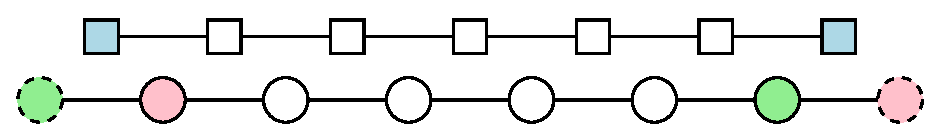
\includegraphics[width=0.9\textwidth]{\dir/figs/grid_ew.eps}
  \caption{A row of the numeric grid when the model is used in torus mode. Circles indicate points in $(i,j)$--grid and squares indicate points in the $(r,s)$--grid. Points with the same color are logically the same.}
  \label{num.fig.grid_ew}
\end{figure}

These boundary conditions are enforced by exchanging points for the temperature and vertical velocity calculations. The ice thicknesses are calculated explicitly at the ghostpoints.

\subsubsection{$\sigma$--Coordinate System}\label{num.sec.sigma}
The vertical coordinate, $z$, is scaled by the ice thickness analogous to the $s$--coordinate in numerical weather simulations \citep[e.g.,][]{Holton1992}. A new vertical coordinate, $\sigma$, is introduced so that the ice surface is at $\sigma=0$ and the ice base at $\sigma=1$ (see Fig. \ref{kin.fig.scale}), i.e.
\begin{equation}
  \label{kin.eq.vertical_scale}
  \sigma=\frac{s-z}{H}.
\end{equation}

\begin{figure}[htbp]
  \begin{center}
    
\includegraphics{\dir/figs/scale.eps}
    \caption[Vertical scaling of the ice sheet model.]{Vertical scaling of the ice sheet model. The vertical axis is scaled to unity. The horizontal coordinates are not changed.}
    \label{kin.fig.scale}
  \end{center}
\end{figure}


The derivatives of a function $f$ in $(x,y,z,t)$ become in the new $(\tilde{x},\tilde{y},\sigma,\tilde{t})$ system:
\begin{subequations}
  \begin{align}
    \frac{\pd f}{\pd x} &= \frac{\pd f}{\pd\tilde{x}}+\frac1H\Delta_{\tilde{x}}\frac{\pd f}{\pd \sigma},\\
    \frac{\pd f}{\pd y} &= \frac{\pd f}{\pd\tilde{y}}+\frac1H\Delta_{\tilde{y}}\frac{\pd f}{\pd \sigma},\\
    \frac{\pd f}{\pd t} &= \frac{\pd f}{\pd\tilde{t}}+\frac1H\Delta_{\tilde{t}}\frac{\pd f}{\pd \sigma},\\
    \frac{\pd f}{\pd z} &= -\frac1H\frac{\pd f}{\pd\sigma},
  \end{align}
\end{subequations}
where  the geometric factors, $\Delta_{\tilde{x}}$, $\Delta_{\tilde{y}}$ and $\Delta_{\tilde{t}}$, are defined by
\begin{subequations}
  \begin{align}
  \Delta_{\tilde{x}}&=\left(\frac{\pd s}{\pd\tilde{x}}-\sigma\frac{\pd H}{\pd\tilde{x}}\right),\\
  \Delta_{\tilde{y}}&=\left(\frac{\pd s}{\pd\tilde{y}}-\sigma\frac{\pd H}{\pd\tilde{y}}\right),\\
  \Delta_{\tilde{t}}&=\left(\frac{\pd s}{\pd\tilde{t}}-\sigma\frac{\pd H}{\pd\tilde{t}}\right).
  \end{align}
\end{subequations}
The integral of $z$ becomes in the $\sigma$--coordinate system:
\begin{equation}
  \int_b^zfdz=-H\int_1^\sigma fd\sigma.
\end{equation}

The vertical coordinate can be discretized using an irregular grid spacing to reflect the fact that ice flow is more variable at the bottom of the ice column. In the vertical the index $k$ is used. 


\subsection{Ice Sheet Equations in $\sigma$--Coordinates}
The horizontal velocity, Equation \eqref{kin.eq.horiz_velo}, becomes in the $\sigma$--coordinate system
\begin{equation}
  \label{kin.eq.vert_velo_sigma}
  \vec u(\sigma) = -2(\rho g)^nH^{n+1}|\vec\nabla s|^{n-1}\vec\nabla s\int_1^\sigma A\sigma^nd\sigma+\vec u(1)
\end{equation}
and the vertically averaged velocity
\begin{equation}
  \label{kin.eq.avg_velo_scaled}
  \overline{\vec u} H=H\int_0^1\vec ud\sigma+\vec u(1)H
\end{equation}
The vertical velocity, Equation \eqref{kin.eq.vert_velo}, becomes
\begin{equation}
  \label{kin.eq.vert_velo_scaled}
  w(\sigma)=-\int_1^\sigma\left(\frac{\pd\vec u}{\pd\sigma}\cdot(\vec\nabla s-\sigma\vec\nabla H)+H\vec\nabla\cdot\vec u\right)d\sigma+w(1)
\end{equation}
and lower boundary condition
\begin{equation}
  w(1)=\frac{\pd h}{\pd t}+\vec u(1)\cdot\vec\nabla h+S.
\end{equation}

\subsection{Calculating the Horizontal Velocity and the Diffusivity}
Horizontal velocity and diffusivity calculations are split up into two parts:
\begin{subequations}
  \label{kin.eq.horiz_diffusivity}
  \begin{align}
    \vec u(\sigma)&=c\vec\nabla s+\vec u(1)\\
    D &=H\int_0^1cd\sigma\\
    \vec q&=D\vec\nabla s+H\vec u(1)\\
    \intertext{with}
    c(\sigma)&=-2(\rho g)^nH^{n+1}|\vec\nabla s|^{n-1}\int_1^\sigma A\sigma^nd\sigma
  \end{align}
\end{subequations}

Quantities $\vec u$ and $D$ are found on the velocity grid. Integrating from the ice base ($k=N-1$), the discretised quantities become
\begin{subequations}
  \begin{equation}
    \tilde{c}_{r,s,N}=0
  \end{equation}
  \begin{multline}
    \tilde{c}_{r,s,k}=-2(\rho g)^nH_{r,s}^{n+1}\left(({\tilde{s}^x_{r,s}})^2+({\tilde{s}^y_{r,s}})^2\right)^{\frac{n-1}{2}}\\
    \sum_{\kappa=N-1}^k\frac{A_{r,s,\kappa}+A_{r,s,\kappa+1}}2 \left(\frac{\sigma_{\kappa+1}+\sigma_\kappa}2\right)^n(\sigma_{\kappa+1}-\sigma_\kappa)
  \end{multline}
  \begin{equation}
    \tilde{D}_{r,s}=H_{r,s}\sum_{k=0}^{N-1}\frac{\tilde{c}_{r,s,k}+\tilde{c}_{r,s,k+1}}2(\sigma_{k+1}-\sigma_k)
  \end{equation}
\end{subequations}
Expressions for $\vec{u}_{i,j,k}$ and $\vec{q}_{i,j}$ are straight forward.

\subsection{Solving the Ice Thickness Evolution Equation}
Equation \eqref{kin.eq.ice_thickness} can be rewritten as a diffusion equation, with non--linear diffusion coefficient $D$:
\begin{equation}
  \label{kin.eq.ice_evo}
  \frac{\pd H}{\pd t}=-\vec\nabla\cdot D\vec\nabla s+B=-\vec\nabla\cdot\vec q+B
\end{equation}
This non--linear partial differential equation can be linearised by using the diffusion coefficient from the previous time step. The diffusion coefficient is calculated on the $(r,s)$--grid, i.e. staggered in both $x$ and $y$ direction. Figure \ref{kin.fig.staggered_grid} illustrates the staggered grid. Using finite differences, the fluxes in $x$ direction, $q^x$ become
\begin{subequations}
\begin{align}
  q^x_{i+\frac12,j}&=-\frac12(\tilde{D}_{r,s}+\tilde{D}_{r,s-1})\frac{s_{i+1,j}-s_{i,j}}{\Delta x}\\
  q^x_{i-\frac12,j}&=-\frac12(\tilde{D}_{r-1,s}+\tilde{D}_{r-1,s-1})\frac{s_{i,j}-s_{i-1,j}}{\Delta x}\\
  \intertext{and the fluxes in $y$ direction}
  q^y_{i,j+\frac12}&=-\frac12(\tilde{D}_{r,s}+\tilde{D}_{r-1,s})\frac{s_{i,j+1}-s_{i,j}}{\Delta y}\\
  q^y_{i,j-\frac12}&=-\frac12(\tilde{D}_{r,s-1}+\tilde{D}_{r-1,s-1})\frac{s_{i,j}-s_{i,j-1}}{\Delta y}.
\end{align}  
\end{subequations}

\begin{figure}[htbp]
  \centering
  
\includegraphics{\dir/figs/staggered_grid.eps}
  \caption{Illustration of the staggered grid used to calculate ice thicknesses, diffusivities and mass fluxes.}
  \label{kin.fig.staggered_grid}
\end{figure}

\subsubsection{ADI Scheme}
The alternating--direction implicit method (ADI) uses the concept of operator splitting where Equation \eqref{kin.eq.ice_evo} is first solved in the $x$--direction and then in the $y$--direction, \citep{Press1992}. The time step $\Delta t$ is devided into two time steps $\Delta t/2$. The descretised version of Equation \eqref{kin.eq.ice_evo} becomes \citep{Huybrechts1986}:
\begin{subequations}
\begin{align}
  \label{kin.eq.adi_1}
  2\frac{H_{i,j}^{t+\frac12}-H_{i,j}^{t}}{\Delta t} &= -\frac{q_{i+\frac12,j}^{x,t+\frac12}-q_{i-\frac12,j}^{x,t+\frac12}}{\Delta x} - \frac{q_{i,j+\frac12}^{y,t}-q_{i,j-\frac12}^{y,t}}{\Delta y} + B_{i,j} \\
  \label{kin.eq.adi_2}
  2\frac{H_{i,j}^{t+1}-H_{i,j}^{t+\frac12}}{\Delta t} &= -\frac{q_{i+\frac12,j}^{x,t+\frac12}-q_{i-\frac12,j}^{x,t+\frac12}}{\Delta x} - \frac{q_{i,j+\frac12}^{y,t+1}-q_{i,j-\frac12}^{y,t+1}}{\Delta y} + B_{i,j}
\end{align}
\end{subequations}
Gathering all $t+\frac12$ terms on the left side, Equation \eqref{kin.eq.adi_1} can be expressed as a tri--diagonal set of equations for each row $j$:
\begin{equation}
  -\alpha_{i,j}H_{i-1,j}^{t+\frac12} + (1-\beta_{i,j})H_{i,j}^{t+\frac12} - \gamma_{i,j}H_{i+1,j}^{t+\frac12} = \delta_{i,j}
\end{equation}
with
\begin{subequations}
  \begin{align}
  \alpha_{i,j} &=\frac{\tilde{D}_{r-1,s}+\tilde{D}_{r-1,s-1}}{4\Delta x^2}\Delta t\\
  \beta_{i,j}  &=-\frac{\tilde{D}_{r,s}+2\tilde{D}_{r-1,s}+\tilde{D}_{r-1,s-1}}{4\Delta x^2}\Delta t = -(\alpha_{i,j}+\gamma_{i,j})\\
  \gamma_{i,j} &=\frac{\tilde{D}_{r,s}+\tilde{D}_{r,s-1}}{4\Delta x^2}\Delta t    
  \end{align}
and the RHS,
\begin{equation}
  \delta_{i,j} = H_{i,j}^t-\frac{\Delta t}{2\Delta y}\left(q_{i,j+\frac12}^{y,t}-q_{i,j-\frac12}^{y,t}\right) + \frac{\Delta t}2B_{i,j} + \alpha_{i,j}h_{i-1,j} -\beta_{i,j}h_{i,j} + \gamma_{i,j}h_{i+1,j}.
\end{equation}
\end{subequations}

A similar tri--diagonal system is found for each column, $i$ of Equation \eqref{kin.eq.adi_2}.

\subsubsection{Linearised Semi--Implicit Scheme}
Using the Crank--Nicolson scheme, the semi--implicit temporal discretisation of \eqref{kin.eq.ice_evo} is then:
\begin{multline}
\label{kin.eq.ice_evo_disc1}
  \frac{H^{t+1}_{i,j}-H^t_{i,j}}{\Delta t}=\frac{q^{x,t+1}_{i+\frac12,j}-q^{x,t+1}_{i-\frac12,j}}{2\Delta x}+\frac{q^{y,t+1}_{i,j+\frac12}-q^{y,t+1}_{i,j-\frac12}}{2\Delta y} \\
  +\frac{q^{x,t}_{i+\frac12,j}-q^{x,t}_{i-\frac12,j}}{2\Delta x}+\frac{q^{y,t}_{i,j+\frac12}-q^{y,t}_{i,j-\frac12}}{2\Delta y}+ B_{i,j}
\end{multline}
The superscripts $^t$ and $^{t+1}$ indicate at what time the ice thickness $H$ is evaluated. Collecting all $H^{t+1}$ terms of \eqref{kin.eq.ice_evo_disc1} on the LHS and moving all other terms to the RHS we can rewrite \eqref{kin.eq.ice_evo_disc1} as
\begin{equation}
  \label{kin.eq.evo_matrix}
  -\alpha_{i,j}H^{t+1}_{i-1,j} - \beta_{i,j}H^{t+1}_{i+1,j} - \gamma_{i,j}H^{t+1}_{i,j-1} - \delta_{i,j}H^{t+1}_{i,j+1}+ (1-\epsilon_{i,j})H^{t+1}_{i,j} = \zeta_{i,j}
\end{equation}
with the RHS,
\begin{multline}
  \zeta_{i,j} = \alpha_{i,j}H^{t}_{i-1,j} + \beta_{i,j}H^{t}_{i+1,j} + \gamma_{i,j}H^{t}_{i,j-1} + \delta_{i,j}H^{t}_{i,j+1} + (1+\epsilon_{i,j})H^{t}_{i,j} \\
  + 2(\alpha_{i,j}h_{i-1,j} + \beta_{i,j}h_{i+1,j} + \gamma_{i,j}h_{i,j-1} + \delta_{i,j}h_{i,j+1}+ \epsilon_{i,j}h_{i,j}) + B_{i,j}\Delta t
\end{multline}
with the elements of the sparse matrix
\begin{subequations}
  \begin{align}
    \alpha_{i,j} &=\frac{\tilde{D}_{r-1,s}+\tilde{D}_{r-1,s-1}}{4\Delta x^2}\Delta t\\
    \beta_{i,j} &=\frac{\tilde{D}_{r,s}+\tilde{D}_{r,s-1}}{4\Delta x^2}\Delta t\\
    \gamma_{i,j} &=\frac{\tilde{D}_{r,s-1}+\tilde{D}_{r-1,s-1}}{4\Delta y^2}\Delta t\\
    \delta_{i,j} &=\frac{\tilde{D}_{r,s}+\tilde{D}_{r-1,s}}{4\Delta y^2}\Delta t\\
    \epsilon_{i,j} &=-(\alpha_{i,j}+\beta_{i,j}+\gamma_{i,j}+\delta_{i,j})
  \end{align}
\end{subequations}

This matrix equation is solved using an iterative matrix solver for non-symmetric sparse matrices. The solver used here is the bi--conjugate gradient method with incomplete LU decomposition preconditioning provided by the SLAP package.

\subsubsection{Non--Linear Scheme}
The non--linearity of Equation \eqref{kin.eq.ice_evo} arises from the dependance of $D$ on $s$. A non--linear scheme for \eqref{kin.eq.ice_evo} can be formulated using Picard iteration, which consists of two iterations: an outer, non--linear and an inner, linear equation. The scheme is started off with the diffusivity from the previous time step, i.e.
\begin{subequations}
  \begin{equation}
    D^{(0),t+1}=D^{t}
  \end{equation}
and Equation \eqref{kin.eq.evo_matrix} becomes
\begin{multline}
  \label{kin.eq.evo_matrix_nonlin}
  -\alpha^{(\xi),t+1}_{i,j}H^{t+1}_{i-1,j} - \beta^{(\xi),t+1}_{i,j}H^{(\xi+1),t+1}_{i+1,j} - \gamma^{(\xi),t+1}_{i,j}H^{(\xi+1),t+1}_{i,j-1} \\
  - \delta^{(\xi),t+1}_{i,j}H^{(\xi+1),t+1}_{i,j+1}+ (1-\epsilon^{(\xi),t+1}_{i,j})H^{(\xi+1),t+1}_{i,j} = \zeta^{(0),t}_{i,j}
\end{multline}
\end{subequations}
Equation \eqref{kin.eq.evo_matrix_nonlin} is iterated over $\xi$ until the maximum ice thickness residual is smaller than some threshold:
\begin{equation}
  \max\left(\left|H^{(\xi+1),t+1}-H^{(\xi),t+1}\right|\right)<H_{\text{res}}
\end{equation}

\begin{figure}[htbp]
  \centering
  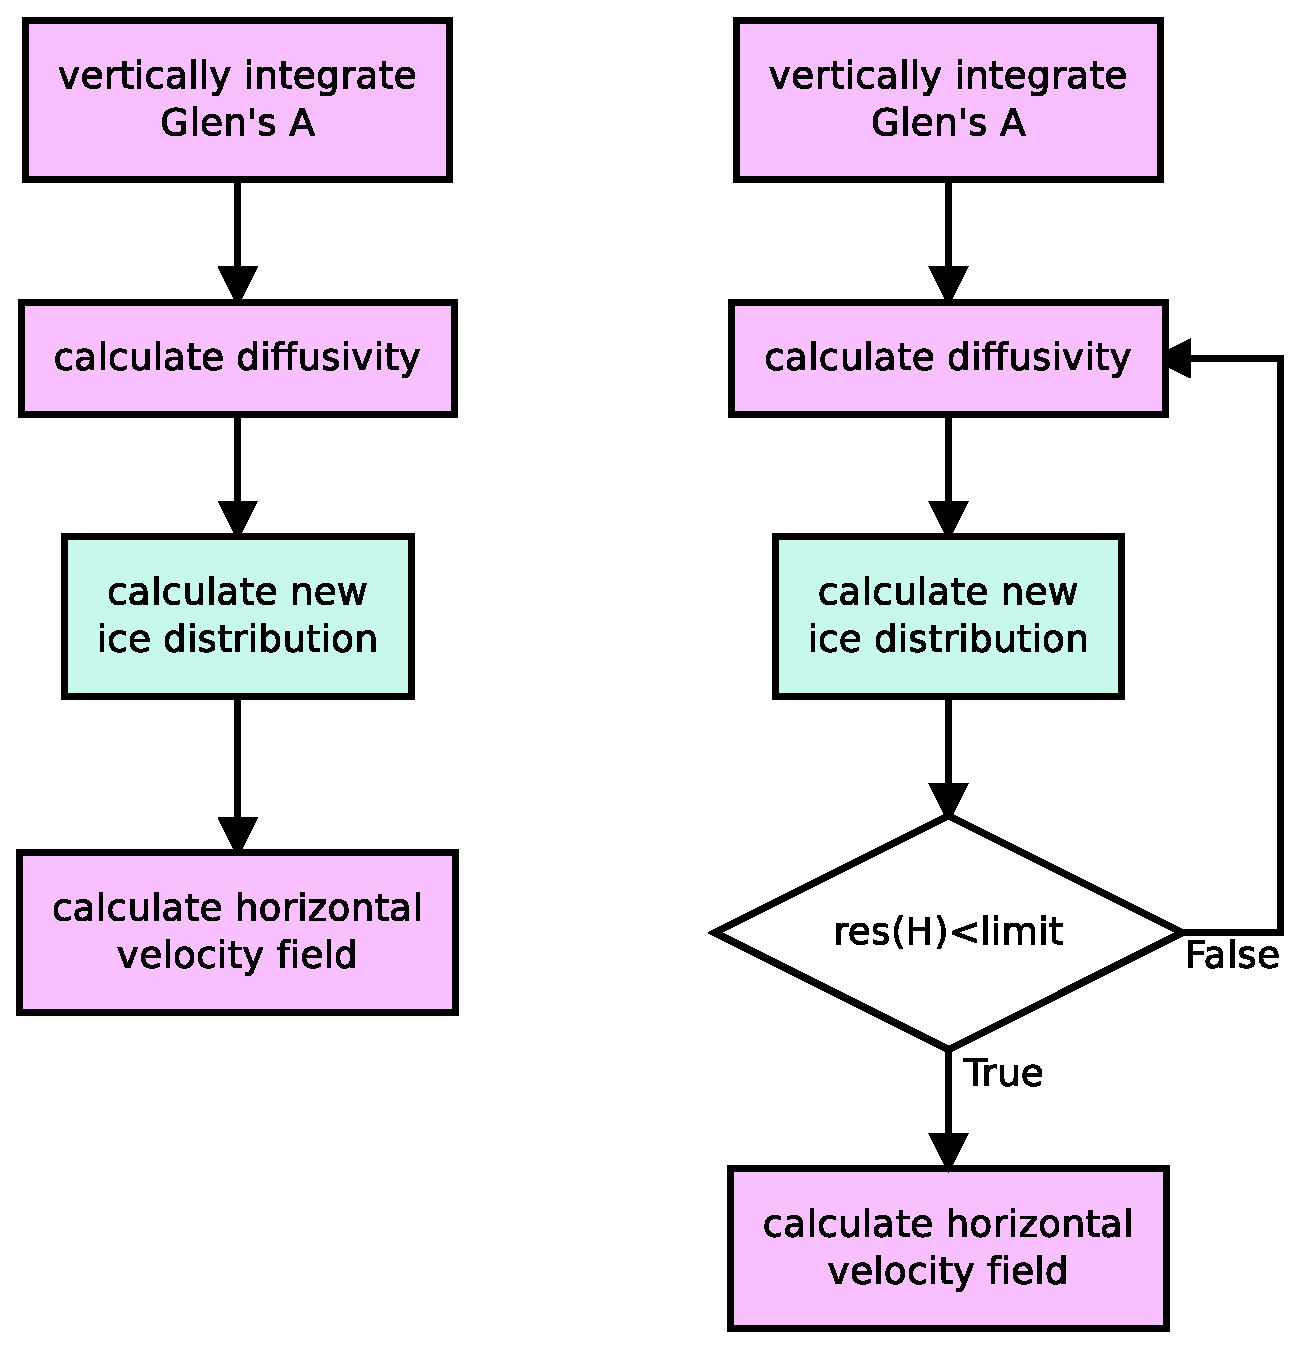
\includegraphics[width=0.5\textwidth]{\dir/figs/thick_evo.eps}
  \caption{Flow diagram showing how the linearised solver (on the left) and the non--linear solver work. The inner, linear iteration is contained within the box labeled ``calculate new ice distribution''.}
  \label{kin.fig.solvers}
\end{figure}

\subsection{Calculating Vertical Velocities}

\subsubsection{Grid Velocity}
The vertical grid moves as a result of using a $\sigma$--coordinate system. The grid velocity is
\begin{equation}
  \label{kin.eq.grid_velo}
  w^{\text{grid}}(\sigma)=\frac{\pd s}{\pd t}+\vec u\cdot\vec\nabla s-\sigma\left(\frac{\pd H}{\pd t}+\vec u\cdot\vec\nabla H\right).
\end{equation}
The numerical implementation of \eqref{kin.eq.grid_velo} is straightforward.

\subsubsection{Vertical Velocity}
The discretized version of the vertical velocity equation \eqref{kin.eq.vert_velo_scaled} is slightly more compilicated because the horizontal velocities are calculated on the $(r,s)$ grid. The vertical velocity at the ice base is $w_{i,j,N}=w^{\text{grid}}_{i,j,N}-M_b{i,j}$, where $M_b{i,j}$ is the basal melt rate. Integrating from the bottom, the vertical velocity is then
\begin{equation}
  \label{kin.eq.wvel_unc}
  \begin{split}
  w_{i,j,k}=-\sum_{\tilde{k}=N-1}^1\left\{\mathcal{H}_{i,j}\left(\frac{u^x_{i,j,k}+u^x_{i,j,k+1}}{2}+\frac{v^y_{i,j,k}+v^y_{i,j,k+1}}{2}\right)(\sigma_{k+1}-\sigma_k)\right. \\
     +(\tilde{u}_{i,j,k+1}-\tilde{u}_{i,j,k})  \left(\tilde{s}^x_{i,j}-\frac12(\sigma_{k+1}+\sigma_k)\tilde{H}^x_{i,j}\right)  \\
     \left.+(\tilde{v}_{i,j,k+1}-\tilde{v}_{i,j,k})  \left(\tilde{s}^y_{i,j}-\frac12(\sigma_{k+1}+\sigma_k)\tilde{H}^y_{i,j}\right)\right\} + w_{i,j,N},
  \end{split}
\end{equation}
with the weighted ice thickness
\begin{equation*}
  \begin{split}
  \mathcal{H}_{i,j}=\frac{4H_{i,j}+2(H_{i-1,j}+H_{i+1,j}+H_{i,j-1}+H_{i,j+1})}{16}\\
  +\frac{H_{i-1,j-1}+H_{i+1,j-1}+H_{i+1,j+1}+H_{i-1,j+1}}{16}.    
  \end{split}
\end{equation*}

This scheme produces vertical velocities at the ice divide which are too small. The vertical velocities on the ice surface are given by the upper kinematic boundary condition \eqref{kin.eq.upper_bc}. Equation \eqref{kin.eq.wvel_unc} can be corrected with
\begin{equation}
  \label{kin.eq.wvel_cor}
   w^\ast_{i,j,k}=w_{i,j,k}-(1-\sigma_k)(w_{i,j,k}-{w_s}_{i,j}),
\end{equation}
where ${w_s}_{i,j}$ is the vertical velocity at the ice surface given by \eqref{kin.eq.upper_bc}. Figure \ref{kin.fig.w_profile} shows the different vertical velocities at the ice surface.
\begin{figure}[htbp]
  \centering
  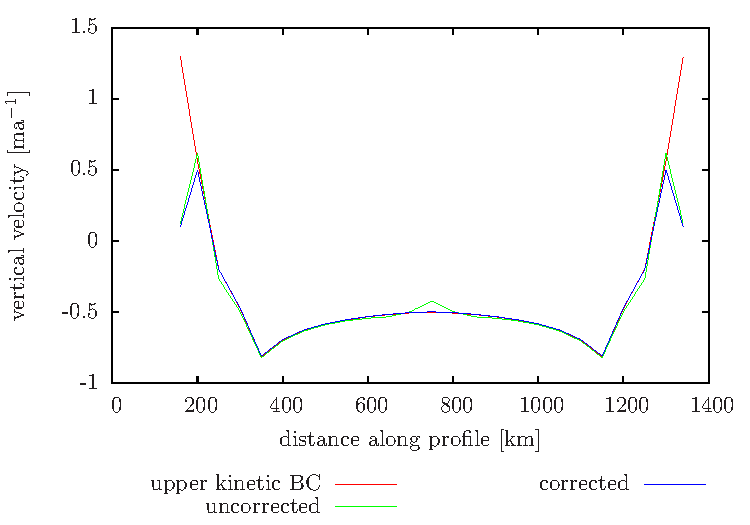
\includegraphics{\dir/gnu/w_profile.eps}
  \caption{Vertical ice surface velocities of the EISMINT-1 moving margin experiment.}
  \label{kin.fig.w_profile}
\end{figure}
The difference between the vertical velocities calculated by the model and the vertical velocities given by \eqref{kin.eq.upper_bc} at the ice margin are due to the fact that temperatures and velocities are only calculated when the ice is thicker than a certain threshold value which is not met at the ice margin.

Figure \ref{kin.fig.wt_sigma} shows vertical profiles of the vertical velocity at the ice divide and a point halfway between the divide and the domain margin. A corresponding temperature profile is also shown since the vertical velocity determines the vertical temperature advection (see Section \ref{temp.sec.vert_ad}).
\begin{figure}[htbp]
  \centering
  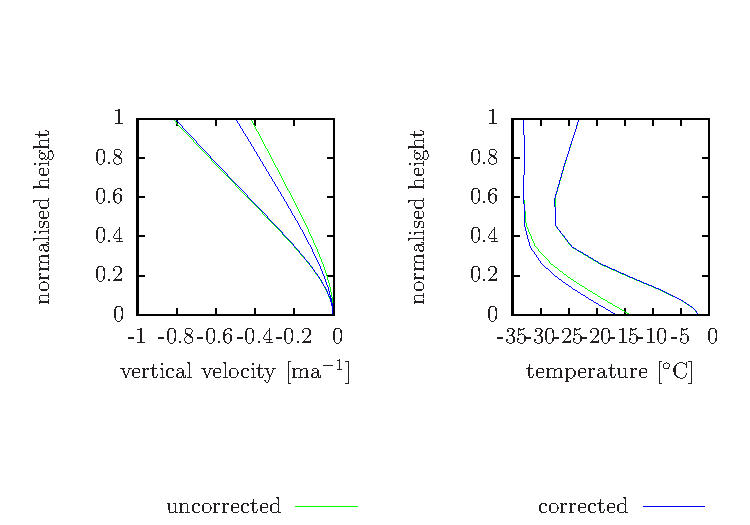
\includegraphics{\dir/gnu/wt_sigma.eps}
  \caption{Vertical velocity and temperature distribution for columns at the ice divide and a point halfway between the divide and the domain margin.}
  \label{kin.fig.wt_sigma}
\end{figure}


\section{Temperature Solver}
The flow law, Equation \eqref{kin.eq.flowlaw}, depends on the temperature of ice. It is, therefore, necessary to determine how the distribution of ice temperatures changes with a changing ice sheet configuration. The thermal evolution of the ice sheet is described by
\begin{equation}
  \label{temp.eq.temp_z}
  \frac{\pd T}{\pd t}=\frac{k}{\rho c}\nabla^2T-\vec{u}\cdot\vec\nabla T+\frac\Phi{\rho c}-w\frac{\pd T}{\pd z},
\end{equation}
where $T$ is the absolute temperature, $k$ is the thermal conductivity of ice, $c$ is the specific heat capacity and $\Phi$ is the heat generated due to internal friction. In the $\sigma$--coordinate system, Equation \eqref{temp.eq.temp_z}, becomes
\begin{equation}
  \label{temp.eq.temp}
  \frac{\pd T}{\pd t} = \frac{k}{\rho cH^2}\frac{\pd^2T}{\pd\sigma^2} - \vec{u}\cdot\vec\nabla T + \frac{\sigma g}c\frac{\pd \vec{u}}{\pd\sigma}\cdot\vec\nabla s + \frac1H\frac{\pd T}{\pd\sigma}\left(w-w_{\text{grid}}\right)
\end{equation}
The terms represents (1) vertical diffusion, (2) horizontal advection, (3) internal heat generation due to friction and (4) vertical advection and a correction due to the sigma coordinate system. Let's rewrite \eqref{temp.eq.temp} to introduce some names:
\begin{equation}
  \label{temp.eq.temp2}
  \frac{\pd T}{\pd t} = a\frac{\pd^2T}{\pd\sigma^2} +b(\sigma) + \Phi(\sigma) + c(\sigma)\frac{\pd T}{\pd\sigma},
\end{equation}
where
\begin{subequations}
  \begin{align}
    a&=\frac{k}{\rho cH^2} \\
    \label{temp.eq.hadv}
    b(\sigma)&=-\vec{u}\cdot\vec\nabla T\\
    \Phi(\sigma)&=\frac{\sigma g}c\frac{\pd \vec{u}}{\pd\sigma}\cdot\vec\nabla s \\
    c(\sigma)&=\frac1H\left(w-w_{\text{grid}}\right)
  \end{align}
\end{subequations}

\subsection{Vertical Diffusion}
Discretisation of $\pd^2T/\pd\sigma^2$ is slightly complicated because the vertical grid is irregular. Using Taylor series the central difference formulas are
\begin{subequations}
  \begin{align}
    \label{temp.eq.d1}
    \left.\frac{\pd T}{\pd\sigma}\right|_{\sigma_{k-1/2}}&=\frac{T_k-T_{k-1}}{\sigma_k-\sigma_{k-1}}\\
    \intertext{and}
    \label{temp.eq.d2}
    \left.\frac{\pd T}{\pd\sigma}\right|_{\sigma_{k+1/2}}&=\frac{T_{k+1}-T_k}{\sigma_{k+1}-\sigma_k}\\
    \intertext{The second partial derivative is then, also using central differences:}
    \label{temp.eq.d3}
    \left.\frac{\pd^2 T}{\pd\sigma^2}\right|_{\sigma_k} &= \frac{\left.{\pd T}/{\pd\sigma}\right|_{\sigma_{k+1/2}} - \left.{\pd T}/{\pd\sigma}\right|_{\sigma_{k-1/2}}}{1/2\left(\sigma_{k+1}-\sigma_{k-1}\right)}\\
    \intertext{Inserting \eqref{temp.eq.d1} and \eqref{temp.eq.d2} into \eqref{temp.eq.d3}, we get:}
    \label{temp.eq.d4}
    &=\frac{2(T_{k+1}-T_k)}{(\sigma_{k+1}-\sigma_k)(\sigma_{k+1}-\sigma_{k-1})}-\frac{2(T_k-T_{k-1})}{(\sigma_k-\sigma_{k-1})(\sigma_{k+1}-\sigma_{k-1})}
  \end{align}
\end{subequations}
Finally, the terms of equation \eqref{temp.eq.d4} are rearranged:
\begin{multline}
  \label{temp.eq.dsigma2}
  \left.\frac{\pd^2 T}{\pd\sigma^2}\right|_{\sigma_k} = \frac{2T_{k-1}}{(\sigma_k-\sigma_{k-1})(\sigma_{k+1}-\sigma_{k-1})} - \frac{2T_k}{(\sigma_{k+1}-\sigma_k)(\sigma_k-\sigma_{k-1})}\\
  + \frac{2T_{k+1}}{(\sigma_{k+1}-\sigma_k)(\sigma_{k+1}-\sigma_{k-1})}
\end{multline}

\subsection{Horizontal Advection}
The horizontal advection term, $- \vec{u}\cdot\vec\nabla T$ is solved using an upwinding scheme. Let's start with the 1--dimensional case. The method discussed can be straightforwadly extented to 2D. As always, the temperature function is expressed as a Taylor series.
\begin{subequations}
  \begin{align}
    \label{temp.eq.taylor1}
    T(x+\Delta x) &=T(x)+\Delta xT'(x)+\frac{\Delta x^2}2T''(x)+\ldots\\
    \intertext{If we subsitute $\Delta x$ with $2\Delta x$, Equation \eqref{temp.eq.taylor1}}
    \label{temp.eq.taylor2}
    T(x+2\Delta x) &=T(x)+2\Delta xT'(x)+2\Delta x^2T''(x)+\ldots
  \end{align}
\end{subequations}
From \eqref{temp.eq.taylor1} and \eqref{temp.eq.taylor2} we can construct a difference formula where the $\mathcal{O}(\Delta x^2)$ error is cancelled, by multiplying \eqref{temp.eq.taylor1} with 4 and substracting the result from \eqref{temp.eq.taylor2}:
\begin{subequations}
  \begin{align}
    \label{temp.eq.forward_h3}
    T_+'(x)&=\frac{4T(x+\Delta x)-T(x+2\Delta x)-3T(x)}{2\Delta x}\\
    \intertext{and similarly for the backward difference:}
    T_-'(x)&=-\frac{4T(x-\Delta x)-T(x-2\Delta x)-3T(x)}{2\Delta x}
    \end{align}
\end{subequations}
So the horizontal advection term in one dimensions becomes:
\begin{equation}
  b_x = -u_x\frac{\pd T}{\pd x}=\frac{-u_x}{2\Delta x}
  \begin{cases}
    -(4T_{i-1}-T_{i-2}-3T_i) & \text{when $u_x>0$} \\
    4T_{i+1}-T_{i+2}-3T_i & \text{when $u_x<0$} \\
  \end{cases}
\end{equation}
A similar expression is found for $b_y$ by simply substituting $y$ for $x$. Finally, the combined horizontal advection term, is simply
\begin{equation}
  b=-\vec{u}\cdot\vec\nabla T=-\left(u_x\frac{\pd T}{\pd x}+u_y\frac{\pd T}{\pd y}\right)=b_x+b_y=b_1+b_2T_i
\end{equation}

\subsection{Heat Generation}
Taking the derivative of \eqref{kin.eq.vert_velo_sigma} with respect to $\sigma$, we get
\begin{equation}
  \frac{\pd u_x}{\pd\sigma} = -2(\rho g)^nH^{n+1}|\vec\nabla s|^{n-1}\frac{\pd s}{\pd x}A(T^\ast)\sigma^n
\end{equation}
Thus,
\begin{equation}
\begin{split}
  \Phi(\sigma) &= \frac{\sigma g}c\frac{\pd \vec{u}}{\pd\sigma}\cdot\vec\nabla s  = \frac{\sigma g}c\left(\frac{\pd u_x}{\pd \sigma}\frac{\pd s}{\pd x} + \frac{\pd u_y}{\pd \sigma}\frac{\pd s}{\pd y}\right)\\
       &= -2(\rho g)^nH^{n+1}|\vec\nabla s|^{n-1}\frac{\sigma g}cA(T^\ast)\sigma^n \left(\left(\frac{\pd s}{\pd x}\right)^2+\left(\frac{\pd s}{\pd y}\right)^2\right) \\
       &= -\frac2{c\rho}(g\sigma\rho)^{n+1}\left(H|\vec\nabla s|\right)^{n+1}A(T^\ast)
\end{split}  
\end{equation}

The constant factor $\frac2{c\rho}(g\sigma\rho)^{n+1}$ is calculated during initialisation in the subroutine \texttt{init\_temp}. This factor is assigned to array \texttt{c1(1:upn)}. \texttt{c1} also includes various scaling factors and the factor $1/16$ to normalise $\mathcal{A}$.

The next factor, $\left(H|\vec\nabla s|\right)^{n+1}$ is calculated in the subroutine \texttt{finddisp}:
\begin{equation}
  {c_2}_{i,j} = \left(\tilde{H}_{i,j}\sqrt{\tilde{S_x}_{i,j}^2+\tilde{S_y}_{i,j}^2}\right)^{n+1},
\end{equation}


The final factor is found by averaging over the neighbouring nodes:
\begin{equation}
  \mathcal{A}_{i,j}=4A_{i,j}+2(A_{i-1,j}+A_{i+1,j}+A_{i,j-1}+A_{i,j+1})+(A_{i-1,j-1}+A_{i+1,j-1}+A_{i+1,j+1}+A_{i-1,j+1})
\end{equation}

\subsection{Vertical Advection}\label{temp.sec.vert_ad}
The vertical advection term, $\pd T/\pd\sigma$ is solved using the central difference formula for unevenly spaced nodes:
\begin{equation}
  \frac{\pd T}{\pd\sigma}=\frac{T_{k+1}-T_{k-1}}{\sigma_{k+1}-\sigma_{k-1}}
\end{equation}

\subsection{Boundary Conditions}
At the upper boundary, ice temperatures are set to the surface temperature, $T_{\text{surf}}$. The ice at the base is heated by the geothermal heat flux and sliding friction:
\begin{equation}
  \left.\frac{\pd T}{\pd\sigma}\right|_{\sigma=1}=-\frac{GH}k-\frac{H\vec{\tau}_b\cdot\vec{u}(1)}k,
\end{equation}
where $\vec{\tau}_b=-\rho gH\vec\nabla s$ is the basal shear stress and $\vec{u}(1)$ is the basal ice velocity. Ice temperatures are held constant if they reach the pressure melting point of ice, i.e.
\begin{equation}
  T^\ast=T_{\text{pmp}} \quad\text{if $T\ge T_{\text{pmp}}$}.
\end{equation}
Excess heat is then used to formulate a melt rate, $S$:
\begin{equation}
  \label{temp.eq.meltrate}
  S=\frac{k}{\rho L}\left(\frac{\pd T^\ast}{\pd z}-\frac{\pd T}{\pd z}\right),
\end{equation}
where $L$ is the specific latent heat of fusion. Finally, basal temperatures are held constant, if the ice is floating:
\begin{equation}
  \frac{\pd T(1)}{\pd t}  = 0.
\end{equation}


\subsection{Putting it all together}
Equation \eqref{temp.eq.temp} is solved for each ice column. The horizontal dependency of the horizontal advection term, \eqref{temp.eq.hadv}, is resolved by iterating the vertical solution. Putting the individual terms together using a fully explicit finite differences scheme, Equation \eqref{temp.eq.temp2} becomes
\begin{subequations}
  \begin{multline}
    \label{temp.eq.temp3a}
    \frac{T_{k,t+1}-T_{k,t}}{\Delta t} = \left(\frac{2aT_{k-1,t}}{(\sigma_k-\sigma_{k-1})(\sigma_{k+1}-\sigma_{k-1})} - \frac{2aT_{k,t}}{(\sigma_{k+1}-\sigma_k)(\sigma_k-\sigma_{k-1,t})}\right. \\
    \left.+ \frac{2aT_{k+1,t}}{(\sigma_{k+1}-\sigma_k)(\sigma_{k+1}-\sigma_{k-1})}\right)+{b_1}_{k,t}+{b_2}_kT_{k,t}+\Phi_k+c_k\frac{T_{k+1,t}-T_{k-1,t}}{\sigma_{k+1}-\sigma_{k-1}}
\end{multline}
and similarly the fully implicit scheme
  \begin{multline}
    \label{temp.eq.temp3b}
    \frac{T_{k,t+1}-T_{k,t}}{\Delta t} = \left(\frac{2aT_{k-1,t+1}}{(\sigma_k-\sigma_{k-1})(\sigma_{k+1}-\sigma_{k-1})} - \frac{2aT_{k,t+1}}{(\sigma_{k+1}-\sigma_k)(\sigma_k-\sigma_{k-1,t+1})}\right. \\
    \left.+ \frac{2aT_{k+1,t+1}}{(\sigma_{k+1}-\sigma_k)(\sigma_{k+1}-\sigma_{k-1})}\right)+{b_1}_{k,t+1}+{b_2}_kT_{k,t+1}+\Phi_k+c_k\frac{T_{k+1,t+1}-T_{k-1,t+1}}{\sigma_{k+1}-\sigma_{k-1}}
\end{multline}
\end{subequations}
Taking the average of Equations \eqref{temp.eq.temp3a} and \eqref{temp.eq.temp3b} gives the \emph{Crank--Nicholson scheme}. The resulting equation is then rearranged and terms of $T_{k-1,t+1}$, $T_{k,t+1}$ and $T_{k+1,t+1}$ are combined to give the tri--diagonal system
\begin{equation}
  \alpha_kT_{k-1,t+1}+\beta_kT_{k,t+1}+\gamma_kT_{k+1,t+1}=\delta_k
\end{equation}
where, for $k=2,N-1$
\begin{subequations}
  \begin{align}
    \alpha_k &= -\frac12\frac{2a\Delta t}{(\sigma_k-\sigma_{k-1})(\sigma_{k+1}-\sigma_{k-1})}+\frac12\frac{c_k\Delta t}{\sigma_{k+1}-\sigma_{k-1}} \\
    \beta_k &= 1+\frac12\frac{2a\Delta t}{(\sigma_{k+1}-\sigma_k)(\sigma_k-\sigma_{k-1})}-\frac12{b_2}_k\Delta t=1-\alpha_k-\gamma_k-\frac12{b_2}_k\Delta t\\
    \gamma_k &= -\frac12\frac{2a\Delta t}{(\sigma_{k+1}-\sigma_k)(\sigma_{k+1}-\sigma_{k-1})}-\frac12\frac{c_k\Delta t}{\sigma_{k+1}-\sigma_{k-1}} \\
    \delta_k &= -\alpha_kT_{k-1,t}+(2-\beta_k)T_{k,t}-\gamma_kT_{k+1,t}+\frac12({b_1}_{k,t}+{b_1}_{k,t+1})\Delta t+\Phi_k\Delta t
  \end{align}

\subsubsection{Boundary Conditions}
At the upper boundary:
\begin{equation}
  \alpha_1=0,\quad\beta_1=1,\quad\gamma_1=0,\quad\delta_1=T_{\text{surf}}
\end{equation}
\end{subequations}


The lower boundary condition is somewhat more complicated. Here we only look at the case when the temperature is below the pressure melting point of ice. BC for floating ice and temperatures at the pressure melting point of ice are trivial. The geothermal heat flux is applied at the lower boundary, i.e. Equation \eqref{temp.eq.d2} becomes
\begin{equation}
  \label{temp.eq.d2-lb}
  \left.\frac{\pd T}{\pd\sigma}\right|_{\sigma_{k+1/2}}=-\frac{GH}k
\end{equation}
Assuming that $\sigma_k-\sigma_{k-1}=\sigma_{k+1}-\sigma_k=\Delta\sigma$ and inserting \eqref{temp.eq.d1} and \eqref{temp.eq.d2-lb} into \eqref{temp.eq.d3}, the second partial derivative becomes
\begin{equation}
  \left.\frac{\pd^2 T}{\pd\sigma^2}\right|_{\sigma_N} = \left(-\frac{GH}k-\frac{T_N-T_{N-1}}{\Delta\sigma}\right)/\Delta\sigma=-\frac{GH}{k\Delta\sigma}-\frac{T_N-T_{N-1}}{\Delta\sigma^2}
\end{equation}
Inserting the new conduction term and replacing the derivative of the vertical advection term with the Neumann boundary condition, Equation \eqref{temp.eq.temp3a} becomes
\begin{subequations}
  \begin{equation}
    \frac{T_{N,t+1}-T_{N,t}}{\Delta t} = -a\left(\frac{GH}{k\Delta\sigma}+\frac{T_{N,t}-T_{N-1,t}}{\Delta\sigma^2}\right)+{b_1}_{N,t}+{b_2}_NT_{N,t}+\Phi_N-c_N\frac{GH}k
  \end{equation}
  and similarly for Equation \eqref{temp.eq.temp3b}
  \begin{multline}
    \frac{T_{N,t+1}-T_{N,t}}{\Delta t} = -a\left(\frac{GH}{k\Delta\sigma}+\frac{T_{N,t+1}-T_{N-1,t+1}}{\Delta\sigma^2}\right)+{b_1}_{N,t+1}+{b_2}_NT_{N,t+1}\\
    +\Phi_N-c_N\frac{GH}k
  \end{multline}
\end{subequations}
The elements of the tri--diagonal system at the lower boundary are then
\begin{subequations}
  \begin{gather}
    \alpha_N =-\frac{a\Delta t}{2(\sigma_N-\sigma_{N-1})^2}\\
    \beta_N = 1-\alpha_N+\frac12{b_2}_N\Delta t\\
    \gamma_N = 0 \\
    \begin{split}
      \delta_N =&-\alpha_NT_{N-1,t}+(2-\beta_N)T_{N,t}-a\frac{GH\Delta t}{k(\sigma_N-\sigma_{N-1})}\\
      &+\frac12({b_1}_{N,t}+{b_1}_{N,t+1})\Delta t+\Phi_N\Delta t-c_N\frac{GH\Delta t}k
    \end{split}
  \end{gather}
\end{subequations}


\section{Basal Boundary Condition}
This section describes the formulation of the basal boundary condition.
An interface for the upper boundary condition (atmospheric BC) is easily defined by the surface temperature and mass balance. Similarly, the basal boundary consists of mechanical and thermal boundary conditions. The complications arise because the thermal and mechanical boundary conditions depend on each other. The interface of the basal boundary can be described with the following fields (see also Fig. \ref{num.fig.basal_bc}):
\begin{enumerate}
\item \textbf{basal traction:} This field specifies a parameter which is used to allow basal sliding.
\item \textbf{basal heat flux:} This is the heat flux entering the ice sheet from below.
\item \textbf{basal water depth:} The presence of basal melt water affects the basal ice temperature.
\end{enumerate}
Also, the ice sheet model calculates a melt/freeze rate based on the temperature gradient and basal water depth. This is handled by Glide.

\begin{figure}[htbp]
  \centering
  
\includegraphics[width=0.9\textwidth]{\dir/figs/basal_bc.eps}
  \caption{Basal boundary condition.}
  \label{num.fig.basal_bc}
\end{figure}

\subsection{Mechanical boundary conditions}
If the ice is not frozen to the bed, basal d\'{e}collement may occur. This can be parameterized by a traction factor, $t_b$. 
Within the ice sheet model, $t_b$ can be used to calculate basal sliding velocities $\vec{u}_b$ in the case of zero--order physics. That is,
\begin{equation}
  \vec{u}_b=t_b\vec{\tau}_b,
\end{equation}
where $\tau_b$ is the basal shear stress. Alternatively, $t_b$ can be used as part of the stress--balance calculations when the model is used with higher order physics. In simple models $t_b$ may be uniform or prescribed as a spatial variable. More complex models may wish to make $t_b$ dependent on other variables, such as basal melt rate. Typically $t_b$ will depend on the presence of basal water.

The second mechanical boundary condition, basal melting/freeze--on $M_b$, is handled within the ice sheet model. The details are described in Section \ref{num.sec.bc_melt}.

\subsection{Thermal boundary conditions}
The thermal boundary condition at the ice base is more complicated than the mechanical BC. The ice is heated from below by the geothermal heat flux. Heat is generated by friction with the bed. Furthermore, the ice temperature is constrained to be less than or equal to the pressure melting point of ice. The thermal boundary condition is a flux condition if there is no water present. If there is water, the basal temperature is set to the pressure melting temperature. (If it were lower, there would be no water, and if it were higher, there would be no ice.)

\subsubsection{Basal melting and freezing}\label{num.sec.bc_melt}
At the ice base, $z=b$, we can define outgoing and incoming heat fluxes, $H_o$ and $H_i$:
\begin{subequations}
  \begin{align}
    H_o&=-k_{\text{ice}}\left.\frac{\pd T}{\pd z}\right|_{z=b^+}\\
    \intertext{and}
    H_i&=-k_{\text{rock}}\left.\frac{\pd T}{\pd z}\right|_{z=b^-}+\vec{u}_b\cdot\vec{\tau}_b+
    \begin{cases}
      {\rho_{\text{ice}}M_b}/{L} & \text{when $M_b<0$} \\
      0 & \text{otherwise}
    \end{cases}
  \end{align}
\end{subequations}
where $k_{\text{ice}}$ and $k_{\text{rock}}$ are the thermal conductivities of ice and rock, $\vec{u}_b\cdot\vec{\tau}_b$ is the heat generated by friction with the bed, and $L$ is the latent heat of fusion. The basal melt/freeze--on rate $M_b$ can then be calculated from the difference between the incoming and outgoing heat fluxes:
\begin{equation}
  \label{bc.eq.meltrate}
  M_b=\frac{H_i-H_o}{\rho_{\text{ice}}L}
\end{equation}
There is freeze--on if $M_b < 0$, and basal melting if $B_b > 0$.

\subsubsection{Geothermal Heat Flux}
The heat flux accross the basal boundary depends on past temperature variations since temperature perturbations penetrate the bed rock if the ice is frozen to the ground \citep{Ritz1987}. 
The heat equation for the bed rock layer is given by the diffusion equation
\begin{equation}
  \label{num.eq.diffu_rock}
  \frac{\pd T}{\pd t} = \frac{k_{\text{rock}}}{\rho_{\text{rock}}c_{\text{rock}}}\nabla^2T=\frac{k_{\text{rock}}}{\rho_{\text{rock}}c_{\text{rock}}} 
  \left(\frac{\pd^2 T}{\pd x^2}+\frac{\pd^2 T}{\pd y^2}+\frac{\pd^2 T}{\pd z^2}\right),
\end{equation}
where $k_{\text{rock}}$ is the thermal conductivity, $\rho_{\text{rock}}$ the density and $c_{\text{rock}}$ the specific heat capacity of the bed rock layer. 

Initial conditions for the temperature field $T$ are found by applying the geothermal heat flux, $G$ to an arbitrary surface temperature $T_0$:
\begin{equation}
  T(x,y,z)=T_0+\frac{G}{k_{\text{rock}}}z.
\end{equation}
This ensures that initially the geothermal heat flux experienced by the ice sheet is equal to the regional heat flux. The basal boundary condition of the bedrock layer is kept constant, i.e.
\begin{equation}
  T(x,y,H_{\text{rock}})=T_0+\frac{G}{k_{\text{rock}}}H_{\text{rock}}.
\end{equation}
Lateral boundary conditions are given by
\begin{equation}
  \left.\frac{\pd T}{\pd x}\right|_{x=0} = \left.\frac{\pd T}{\pd x}\right|_{x=L_x} = \left.\frac{\pd T}{\pd y}\right|_{y=0} = \left.\frac{\pd T}{\pd y}\right|_{y=L_y} = 0.
\end{equation}
At the upper boundary, the heat flux of the rock layer has to be matched with the heat flux in the basal ice layer when the ice is frozen to the bed, i.e.
\begin{equation}
  \label{num.eq.gthf_bc}
  k_{\text{rock}}\left.\frac{\pd T}{\pd z}\right|_{z=-0}=k_{\text{ice}}\left.\frac{\pd T}{\pd z}\right|_{z=+0}.
\end{equation}
Otherwise the temperature of the top bedrock layer is set to the surface temperature (if the cell has been occupied by ice, but there is no ice present) or the basal ice temperature (if there is ice). Equation \eqref{num.eq.gthf_bc} is automatically fulfilled if we set the top bedrock temperature to the basal ice temperature \emph{everywhere} and then calculate the geothermal heat flux to be used as boundary condition for Equation \eqref{temp.eq.temp_z}.



\subsection{Numerical Solution}
The horizontal grid is described in Section \ref{num.sec.grid}. The vertical grid is irregular like the vertical grid of the ice sheet model. However, it is not scaled. Also for now, I have ignored topography or isostatic adjustment, i.e. the bedrock layer is assumed to be flat and constant.

The horizontal second derivative in Equation \eqref{num.eq.diffu_rock} becomes using finite--differences
\begin{equation}
  \left.\frac{\pd^2T}{\pd x^2}\right|_{x_i,y_i,z_i} = T_{xx,i,j,k} = \frac{T_{i+1,j,k}-2T_{i,j,k}+T_{i-1,j,k}}{\Delta x}
\end{equation}
and similarly for $\pd^2T/\pd y^2$. The vertical second derivative $\pd^2T/\pd z^2$ is similar to Equation \eqref{temp.eq.dsigma2}:
\begin{multline}
  \left.\frac{\pd^2 T}{\pd z^2}\right|_{x_i,y_i,z_i} = T_{zz,i,j,k} = \frac{2T_{i,j,k-1}}{(z_k-z_{k-1})(z_{k+1}-z_{k-1})} - \frac{2T_{i,j,k}}{(z_{k+1}-z_k)(z_k-z_{k-1})}\\
  + \frac{2T_{i,j,k+1}}{(z_{k+1}-z_k)(z_{k+1}-z_{k-1})}
\end{multline}


Using the Crank-Nicholson scheme, Equation \eqref{num.eq.diffu_rock} becomes
\begin{equation}
  \label{num.eq.diffu_rock_disc}
  \frac{T_{i,j,k}^{t+1}-T_{i,j,k}^{t}}{\Delta t}=D\left\{\frac{T_{xx,i,j,k}^{t+1}+T_{xx,i,j,k}^{t}}2 + \frac{T_{yy,i,j,k}^{t+1}+T_{yy,i,j,k}^{t}}2 + \frac{T_{zz,i,j,k}^{t+1}+T_{zz,i,j,k}^{t}}2 \right\},
\end{equation}
with $D=k_{\text{rock}}/(\rho_{\text{rock}}c_{\text{rock}})$. Equation \eqref{num.eq.diffu_rock_disc} is solved by gathering all $T^{t+1}$ terms on the LHS and all other terms on the RHS. The index $(i,j,k)$ is linearised using $\iota = i+(j-1)N+(k-1)NM$. The resulting matrix system is solved using the same bi--conjugate gradient solver as for the ice thickness evolution.



\subsection{Basal hydrology}
It is clear from the discussion above that the presence of basal water plays a crucial role in specifying both the mechanical and thermal boundary conditions. However, the treatment of basal water can vary greatly. Basal water is, therefore, left as an unspecified interface. Glide does provide a simple local water balance model which can be run in the absence of more complex models.

\subsection{Putting it all together}
The basal boundary consists of the individual components described in the previous sections. All components are tightly linked with each other. Figure \ref{num.fig.bc_flow} illustrates how the modules are linked and in what order they are resolved.
\begin{figure}[htbp]
  \centering
  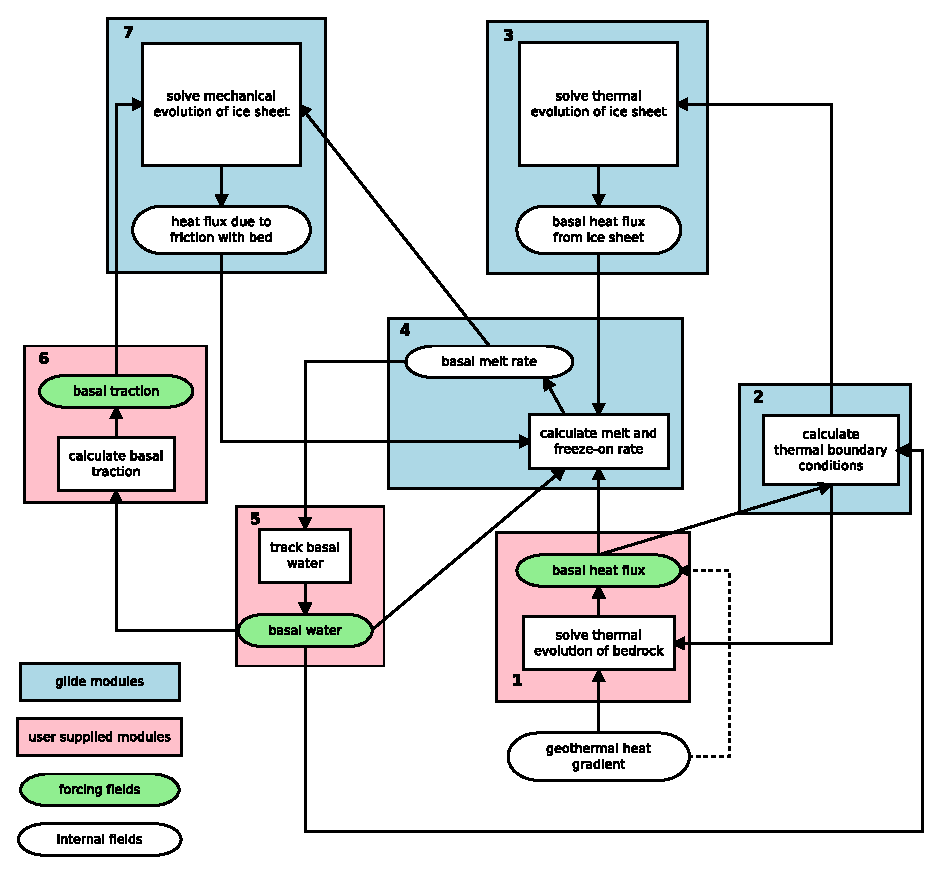
\includegraphics[width=\textwidth]{\dir/figs/basal_alg.eps}
  \caption{Flow diagram illustrating how the various modules communicate with each other by exchanging data fields.}
  \label{num.fig.bc_flow}
\end{figure}
The order of executions is then:
\begin{enumerate}
\item Find the basal heat flux by either solving the equation describing the thermal evolution of the lithosphere, \eqref{num.eq.diffu_rock}, or by using the geothermal heat flux directly. The upper boundary condition of \eqref{num.eq.diffu_rock} is the same as the lower boundary condition of the thermal evolution of the ice sheet.
\item Either (1) the lower boundary condition for the thermal evolution of the ice sheet is given by the basal heat flux from \emph{Step 1}; or (2) if melt water is present, the basal temperature is set to the pressure melting point of ice.
\item Calculate the temperature distribution within the ice sheet given the boundary condition found during \emph{Step 2} and the atmospheric BC.
\item Calculate a melt/freeze--on rate using Equation \eqref{bc.eq.meltrate} given the outgoing heat flux calculated during \emph{Step 3}, friction with the bed (calculated during the previous \emph{Step 7}) and the incoming heat flux from \emph{Step 1}. Freezing occurs only when there is basal water.
\item Track basal water. This is a user supplied module which can take any complexity. Inputs will typically be the melt/freeze--on rate determined during \emph{Step 4}.
\item Calculate the basal traction parameter. Again, this is a user supplied module which typically will involve the presence of basal water (calculated during \emph{Step 5}).
\item Solve the mechanical ice equations given basal traction parameter from \emph{Step 6}.
\end{enumerate}
Clearly, this scheme has the problem that heat is lost if the basal heat flux is such that more water could be frozen than is available. This might be avoided by iterating the process. On the other hand, the heat loss may be negligible if time steps are fairly small.

\section{Isostatic Adjustment}
The ice sheet model includes simple approximations for calculating isostatic adjustment. These approximations depend on how the lithosphere and the mantle are treated. For each subsystem there are two models. The lithosphere can be described as a
\begin{description}
\item[\textbf{local lithosphere:}] the flexural rigidity of the lithosphere is ignored, i.e. this is equivalent to ice floating directly on the asthenosphere;
\item[\textbf{elastic lithosphere:}] the flexural rigidity is taken into account;
\end{description}
while the mantle is treated as a
\begin{description}
\item [\textbf{fluid mantle:}] the mantle behaves like a non-viscous fluid, isostatic equilibrium is reached instantaneously;
\item [\textbf{relaxing mantle:}] the flow within the mantle is approximated by an exponentially decaying hydrostatic response function, i.e. the mantle is treated as a viscous half space.
\end{description}

\subsection{Calculation of ice-water load}
At each isostasy time-step, the load of ice and water is calculated, as an
equivalent mantle-depth ($L$). If the basal elevation is above sea-level, then the
load is simply due to the ice:
\begin{equation}
L=\frac{\rho_i}{\rho_m}H,
\label{load_land_ice}
\end{equation}
where $H$ is the ice thickness, with $\rho_i$ and $\rho_m$ being the densities
of the ice and mantle respectively. In the case where the bedrock is below
sea-level, the load is calculated is that due to a change in sea-level rise and/or
the presence of non-floating ice. When the ice is floating ($\rho_i
H<\rho_o(z_0-h)$), the load is only due to sea-level changes
\begin{equation}
L=\frac{\rho_o}{\rho_m}z_0,
\label{load_sea_float}
\end{equation}
whereas when the ice is grounded, it displaces the water, and adds an
additional load:
\begin{equation}
L=\frac{\rho_i H+\rho_o b_r}{\rho_m}.
\label{load_sea_grounded}
\end{equation}
here, $\rho_o$ is the density of sea water, $z_0$ is the change in sea-level
relative to a reference level and $b_r$ is the bedrock elevation relative to the
same reference level. The value of $b_r$ will be negative for submerged bedrock,
hence the plus sign in (\ref{load_sea_grounded}).

\subsection{Elastic lithosphere model}
This is model is selected by setting \texttt{lithosphere = 1} in the
configuration file. By simulatuing the deformation of the lithosphere, the
deformation seen by the aesthenosphere beneath is calculated. In the absence of this
model, the deformation is that due to Archimedes' Principle, as though the
load were floating on the aesthenosphere.

The elastic lithosphere model is based on work by \cite{Lambeck1980}, and its
implementation is fully described in \cite{Hagdorn2003}. The lithosphere
model only affects the geometry of the deformation --- the timescale for
isostatic adjustment is controlled by the aesthenosphere model. 

The load due to a single (rectangular) grid point is approximated as being
applied to a disc of the same area. The deformation due to a disc of ice of
radius $A$ and thickness $H$ is given by these expressions. For $r<A$:
\begin{equation} 
w(r)=\frac{\rho_i H}{\rho_m}\left[1+C_1\,\mathrm{Ber}\left(\frac{r}{L_r}\right)+C_2\,\mathrm{Bei}\left(\frac{r}{L_r}\right)\right],
\end{equation}
and for $r\geq A$:
\begin{equation}
w(r)=\frac{\rho_i
  H}{\rho_m}\left[D_1\,\mathrm{Ber}\left(\frac{r}{L_r}\right)+D_2\,\mathrm{Bei}\left(\frac{r}{L_r}\right)
+D_3\,\mathrm{Ker}\left(\frac{r}{L_r}\right)+D_4\,\mathrm{Kei}\left(\frac{r}{L_r}\right)\right],
\end{equation}
where $\mathrm{Ber}(x)$, $\mathrm{Bei}(x)$, $\mathrm{Ker}(x)$ and
$\mathrm{Kei}(x)$ are Kelvin functions of zero order, $L_r=(D/\rho_m
g))^{1/4}$ is the radius of relative stiffness, and $D$ is the flexural
rigidity. The constants $C_i$ and $D_i$ are given by
\begin{equation}
\begin{array}{rcl}
C_1&=&a\,\mathrm{Ker}'(a)\\
C_2&=&-a\,\mathrm{Ker}'(a)\\
D_1&=&0\\
D_2&=&0\\
D_3&=&a\,\mathrm{Ber}'(a)\\
D_4&=&-a\,\mathrm{Ber}'(a).
\end{array}
\end{equation}
Here, the prime indicates the first spatial derivative of the Kelvin functions.

\subsection{Relaxing aesthenosphere model}
If a fluid mantle is selected, it adjusts instantly to changes in lithospheric
loading. However, a relaxing mantle is also available.

%%% Local Variables: 
%%% mode: latex
%%% TeX-master: "isos"
%%% End: 



\chapter{Developer Guide}
\renewcommand{\dir}{dg}
\newcommand{\dir}{dg}

\pagestyle{myheadings}
\markright{GLIMMER {\glimmerver} --- Developer's Guide}

\begin{document}
\title{GLIMMER {\glimmerver} --- Developer's Guide}
\author{Magnus Hagdorn\thanks{Magnus.Hagdorn@ed.ac.uk} \and Ian Rutt\thanks{I.C.Rutt@bristol.ac.uk}}
\maketitle
\tableofcontents
\newpage

\newcommand{\dir}{dg}

\pagestyle{myheadings}
\markright{GLIMMER {\glimmerver} --- Developer's Guide}

\begin{document}
\title{GLIMMER {\glimmerver} --- Developer's Guide}
\author{Magnus Hagdorn\thanks{Magnus.Hagdorn@ed.ac.uk} \and Ian Rutt\thanks{I.C.Rutt@bristol.ac.uk}}
\maketitle
\tableofcontents
\newpage

\newcommand{\dir}{dg}

\pagestyle{myheadings}
\markright{GLIMMER {\glimmerver} --- Developer's Guide}

\begin{document}
\title{GLIMMER {\glimmerver} --- Developer's Guide}
\author{Magnus Hagdorn\thanks{Magnus.Hagdorn@ed.ac.uk} \and Ian Rutt\thanks{I.C.Rutt@bristol.ac.uk}}
\maketitle
\tableofcontents
\newpage

\input{\dir/dg.tex}
\end{document}

\end{document}

\end{document}


\renewcommand{\dir}{ext}
\newcommand{\dir}{ext}

\pagestyle{myheadings}

\markright{Glimmer-CISM {\glimmerver} Extension documentation}

\begin{document}
\title{Glimmer-CISM {\glimmerver} Extension Documentation}
\author{Magnus Hagdorn\thanks{Magnus.Hagdorn@ed.ac.uk}, Ian
Rutt\thanks{I.C.Rutt@bristol.ac.uk} \and Tony Payne\thanks{a.j.payne@bristol.ac.uk}}

\maketitle
\tableofcontents
\newpage

\newcommand{\dir}{ext}

\pagestyle{myheadings}

\markright{Glimmer-CISM {\glimmerver} Extension documentation}

\begin{document}
\title{Glimmer-CISM {\glimmerver} Extension Documentation}
\author{Magnus Hagdorn\thanks{Magnus.Hagdorn@ed.ac.uk}, Ian
Rutt\thanks{I.C.Rutt@bristol.ac.uk} \and Tony Payne\thanks{a.j.payne@bristol.ac.uk}}

\maketitle
\tableofcontents
\newpage

\newcommand{\dir}{ext}

\pagestyle{myheadings}

\markright{Glimmer-CISM {\glimmerver} Extension documentation}

\begin{document}
\title{Glimmer-CISM {\glimmerver} Extension Documentation}
\author{Magnus Hagdorn\thanks{Magnus.Hagdorn@ed.ac.uk}, Ian
Rutt\thanks{I.C.Rutt@bristol.ac.uk} \and Tony Payne\thanks{a.j.payne@bristol.ac.uk}}

\maketitle
\tableofcontents
\newpage

\input{\dir/ext.tex}
\bibliography{glimmer}
\end{document}

\bibliography{glimmer}
\end{document}

\bibliography{glimmer}
\end{document}


\part{Appendix}
\appendix
\renewcommand{\dir}{ug}
\chapter{netCDF Variables}
\label{ug.sec.varlist}
The following list shows all the variable names used by GLIMMER. Only variables marked with $^\ast$ are loaded by the input routines.
\section{Glide Variables}
\input{\dir/glide_varlist.tex}
\section{EIS Variables}
\input{\dir/eis_varlist.tex}
\section{GLINT Variables}
\input{\dir/glint_varlist.tex}

\chapter{The GLIMMER API}
\section{GLUM}
GLUM provides some utility subroutines which are shared by all components of GLIMMER.

\subsection{Subroutine \texttt{open\_log}}
\paragraph{Purpose} open and initialise log file

\paragraph{Name and mandatory arguments}
\begin{verbatim}
subroutine open_log
\end{verbatim}

\paragraph{Arguments}
\begin{center}
  \tablefirsthead{%
    \hline
  }
  \tablehead{%
    \hline
    \multicolumn{4}{|p{\textwidth}|}{\emph{\small continued from previous page}}\\
    \hline
  }
  \tabletail{%
    \hline
    \multicolumn{4}{|r|}{\emph{\small continued on next page}}\\
    \hline}
  \tablelasttail{\hline}
  \begin{supertabular*}{\textwidth}{@{\extracolsep{\fill}}lllp{5.5cm}}
    \multicolumn{4}{|l|}{{\bf Mandatory}}\\
    \hline
    \hline
    \multicolumn{4}{|l|}{{\bf Optional}}\\
    \hline
    \texttt{unit} & \texttt{integer} & \texttt{intent(in)} & file unit to use (defualt: 6) \\
    \texttt{fname}& \texttt{character(len=*)} & \texttt{intent(in)} & name of log file (default: \texttt{glide.log})\\ 
  \end{supertabular*}
\end{center}
%%%%%%%%%%%%%%%%%%%%%%%%%%%%%%%%%%%%%%%%%%%%%%%%%%%
\subsection{Subroutine \texttt{ConfigRead}}
\paragraph{Purpose} Read configuration file and store config options.

\paragraph{Name and mandatory arguments}
\begin{verbatim}
subroutine ConfigRead(fname,config)
\end{verbatim}

\paragraph{Arguments}
\begin{center}
  \tablefirsthead{%
    \hline
  }
  \tablehead{%
    \hline
    \multicolumn{4}{|p{\textwidth}|}{\emph{\small continued from previous page}}\\
    \hline
  }
  \tabletail{%
    \hline
    \multicolumn{4}{|r|}{\emph{\small continued on next page}}\\
    \hline}
  \tablelasttail{\hline}
  \begin{supertabular*}{\textwidth}{@{\extracolsep{\fill}}lllp{5.5cm}}
    \multicolumn{4}{|l|}{{\bf Mandatory}}\\
    \hline
    %%
    \texttt{fname} & \texttt{character(len=*)} & \texttt{intent(in)} & name of configuration file to be read\\
    \texttt{config} & \texttt{type(ConfigSection), pointer} & & pointer to first element of linked list containing configuration\\    
  \end{supertabular*}
\end{center}
\paragraph{Additional Notes}
Each section within the configuration file is stored as an element of a linked list. These elements contain another linked list storing the key--value pairs.

%%%%%%%%%%%%%%%%%%%%%%%%%%%%%%%%%%%%%%%%%%%%%%%%%%%
\subsection{Subroutine \texttt{CheckSections}}
\paragraph{Purpose} To check if all sections within a configuration file were subsequently used. Report unused sections to the log.

\paragraph{Name and mandatory arguments}
\begin{verbatim}
subroutine CheckSections(config)
\end{verbatim}
\paragraph{Arguments}
\begin{center}
  \tablefirsthead{%
    \hline
  }
  \tablehead{%
    \hline
    \multicolumn{4}{|p{\textwidth}|}{\emph{\small continued from previous page}}\\
    \hline
  }
  \tabletail{%
    \hline
    \multicolumn{4}{|r|}{\emph{\small continued on next page}}\\
    \hline}
  \tablelasttail{\hline}
  \begin{supertabular*}{\textwidth}{@{\extracolsep{\fill}}lllp{5.5cm}}
    \multicolumn{4}{|l|}{{\bf Mandatory}}\\
    \hline
    %%
    \texttt{config} & \texttt{type(ConfigSection), pointer} & & pointer to first element of linked list containing configuration\\ 
  \end{supertabular*}
\end{center}

%%%%%%%%%%%%%%%%%%%%%%%%%%%%%%%%%%%%%%%%%%%%%%%%%%%
%\subsection{Subroutine \texttt{}}
%\paragraph{Purpose} 
%\paragraph{Name and mandatory arguments}
%\begin{verbatim}
%
%\end{verbatim}
%\paragraph{Arguments}
%\begin{center}
%  \tablefirsthead{%
%    \hline
%  }
%  \tablehead{%
%    \hline
%    \multicolumn{4}{|p{\textwidth}|}{\emph{\small continued from previous page}}\\
%    \hline
%  }
%  \tabletail{%
%    \hline
%    \multicolumn{4}{|r|}{\emph{\small continued on next page}}\\
%    \hline}
%  \tablelasttail{\hline}
%  \begin{supertabular*}{\textwidth}{@{\extracolsep{\fill}}lllp{5.5cm}}
%    \multicolumn{4}{|l|}{{\bf Mandatory}}\\
%    \hline
%    %%
%    \hline
%    \multicolumn{4}{|l|}{{\bf Optional}}\\
%    \hline
%    %%
%  \end{supertabular*}
%\end{center}


\section{GLIDE}\label{ug.sec.glide_api}
%%%%%%%%%%%%%%%%%%%%%%%%%%%%%%%%%%%%%%%%%%%%%%%%%%
\subsection{Subroutine \texttt{glide\_config}}
\paragraph{Purpose} To parse configuration file and print configuration to log
\paragraph{Name and mandatory arguments}
\begin{verbatim}
subroutine glide_config(model,config)
\end{verbatim}
\paragraph{Arguments}
\begin{center}
  \tablefirsthead{%
    \hline
  }
  \tablehead{%
    \hline
    \multicolumn{4}{|p{\textwidth}|}{\emph{\small continued from previous page}}\\
    \hline
  }
  \tabletail{%
    \hline
    \multicolumn{4}{|r|}{\emph{\small continued on next page}}\\
    \hline}
  \tablelasttail{\hline}
  \begin{supertabular*}{\textwidth}{@{\extracolsep{\fill}}lllp{5.5cm}}
    \multicolumn{4}{|l|}{{\bf Mandatory}}\\
    \hline
    %%
    \texttt{model} & \texttt{type(glide\_global\_type)} &\texttt{intent(inout)}& f95 type containing all variables associated with an instance of the model.\\
    \texttt{config} & \texttt{type(ConfigSection), pointer} & & pointer to first element of linked list containing configuration\\ 
  \end{supertabular*}
\end{center}

%%%%%%%%%%%%%%%%%%%%%%%%%%%%%%%%%%%%%%%%%%%%%%%%%%
\subsection{Subroutine \texttt{glide\_initialise}}
\paragraph{Purpose} To initialise the basic ice sheet model
\paragraph{Name and mandatory arguments}
\begin{verbatim}
subroutine glide_initialise(model)
\end{verbatim}
\paragraph{Arguments}
\begin{center}
  \tablefirsthead{%
    \hline
  }
  \tablehead{%
    \hline
    \multicolumn{4}{|p{\textwidth}|}{\emph{\small continued from previous page}}\\
    \hline
  }
  \tabletail{%
    \hline
    \multicolumn{4}{|r|}{\emph{\small continued on next page}}\\
    \hline}
  \tablelasttail{\hline}
  \begin{supertabular*}{\textwidth}{@{\extracolsep{\fill}}lllp{5.5cm}}
    \multicolumn{4}{|l|}{{\bf Mandatory}}\\
    \hline
    %%
    \texttt{model} & \texttt{type(glide\_global\_type)} &\texttt{intent(inout)}& f95 type containing all variables associated with an instance of the model.\\
  \end{supertabular*}
\end{center}
\paragraph{Additional Notes}
This subroutine initialises the model. Memory for all variables is allocated. Input files are opend and read. Output files are created. Variables are scaled.

%%%%%%%%%%%%%%%%%%%%%%%%%%%%%%%%%%%%%%%%%%%%%%%%%%%
\subsection{Subroutine \texttt{glide\_nc\_fillall}}
\paragraph{Purpose} fill netCDF coordinate variables.
\paragraph{Name and mandatory arguments}
\begin{verbatim}
subroutine glide_nc_fillall(model)
\end{verbatim}
\paragraph{Arguments}
\begin{center}
  \tablefirsthead{%
    \hline
  }
  \tablehead{%
    \hline
    \multicolumn{4}{|p{\textwidth}|}{\emph{\small continued from previous page}}\\
    \hline
  }
  \tabletail{%
    \hline
    \multicolumn{4}{|r|}{\emph{\small continued on next page}}\\
    \hline}
  \tablelasttail{\hline}
  \begin{supertabular*}{\textwidth}{@{\extracolsep{\fill}}lllp{5.5cm}}
    \multicolumn{4}{|l|}{{\bf Mandatory}}\\
    \hline
    %%
    \texttt{model} & \texttt{type(glide\_global\_type)} &\texttt{intent(inout)}& f95 type containing all variables associated with an instance of the model.\\
  \end{supertabular*}
\end{center}

%%%%%%%%%%%%%%%%%%%%%%%%%%%%%%%%%%%%%%%%%%%%%%%%%%%
\subsection{Subroutine \texttt{glide\_tstep\_p1}}
\paragraph{Purpose} Performs first part of time-step of an ice model instance: calculate vertical velocity and temperature field. Set model time.
\paragraph{Name and mandatory arguments}
\begin{verbatim}
subroutine glide_tstep_p1(model,time)
\end{verbatim}
\paragraph{Arguments}
\begin{center}
  \tablefirsthead{%
    \hline
  }
  \tablehead{%
    \hline
    \multicolumn{4}{|p{\textwidth}|}{\emph{\small continued from previous page}}\\
    \hline
  }
  \tabletail{%
    \hline
    \multicolumn{4}{|r|}{\emph{\small continued on next page}}\\
    \hline}
  \tablelasttail{\hline}
  \begin{supertabular*}{\textwidth}{@{\extracolsep{\fill}}lllp{5.5cm}}
    \multicolumn{4}{|l|}{{\bf Mandatory}}\\
    \hline
    %%
    \texttt{model} & \texttt{type(glide\_global\_type)} &\texttt{intent(inout)}& f95 type containing all variables associated with an instance of the model.\\
    \texttt{time}  & \texttt{real(rk)} & \texttt{intent(in)} & Current time in years\\
  \end{supertabular*}
\end{center}


%%%%%%%%%%%%%%%%%%%%%%%%%%%%%%%%%%%%%%%%%%%%%%%%%%%
\subsection{Subroutine \texttt{glide\_tstep\_p2}}
\paragraph{Purpose} Performs second part of time-step of an ice model instance: write data and move ice and update horizontal velocities.
\paragraph{Name and mandatory arguments}
\begin{verbatim}
subroutine glide_tstep_p2(model)
\end{verbatim}
\paragraph{Arguments}
\begin{center}
  \tablefirsthead{%
    \hline
  }
  \tablehead{%
    \hline
    \multicolumn{4}{|p{\textwidth}|}{\emph{\small continued from previous page}}\\
    \hline
  }
  \tabletail{%
    \hline
    \multicolumn{4}{|r|}{\emph{\small continued on next page}}\\
    \hline}
  \tablelasttail{\hline}
  \begin{supertabular*}{\textwidth}{@{\extracolsep{\fill}}lllp{5.5cm}}
    \multicolumn{4}{|l|}{{\bf Mandatory}}\\
    \hline
    %%
    \texttt{model} & \texttt{type(glide\_global\_type)} &\texttt{intent(inout)}& f95 type containing all variables associated with an instance of the model.\\
  \end{supertabular*}
\end{center}

%%%%%%%%%%%%%%%%%%%%%%%%%%%%%%%%%%%%%%%%%%%%%%%%%%%
\subsection{Subroutine \texttt{glide\_tstep\_p3}}
\paragraph{Purpose} Performs third part of time-step of an ice model instance: calculate isostatic adjustment and upper and lower ice surface.
\paragraph{Name and mandatory arguments}
\begin{verbatim}
subroutine glide_tstep_p3(model)
\end{verbatim}
\paragraph{Arguments}
\begin{center}
  \tablefirsthead{%
    \hline
  }
  \tablehead{%
    \hline
    \multicolumn{4}{|p{\textwidth}|}{\emph{\small continued from previous page}}\\
    \hline
  }
  \tabletail{%
    \hline
    \multicolumn{4}{|r|}{\emph{\small continued on next page}}\\
    \hline}
  \tablelasttail{\hline}
  \begin{supertabular*}{\textwidth}{@{\extracolsep{\fill}}lllp{5.5cm}}
    \multicolumn{4}{|l|}{{\bf Mandatory}}\\
    \hline
    %%
    \texttt{model} & \texttt{type(glide\_global\_type)} &\texttt{intent(inout)}& f95 type containing all variables associated with an instance of the model.\\
  \end{supertabular*}
\end{center}

%%%%%%%%%%%%%%%%%%%%%%%%%%%%%%%%%%%%%%%%%%%%%%%%%%%
\subsection{Subroutine \texttt{glide\_finalise}}
\paragraph{Purpose} To shut--down model, close all open files and deallocate memory.
\paragraph{Name and mandatory arguments}
\begin{verbatim}
subroutine glide_finalise(model)
\end{verbatim}
\paragraph{Arguments}
\begin{center}
  \tablefirsthead{%
    \hline
  }
  \tablehead{%
    \hline
    \multicolumn{4}{|p{\textwidth}|}{\emph{\small continued from previous page}}\\
    \hline
  }
  \tabletail{%
    \hline
    \multicolumn{4}{|r|}{\emph{\small continued on next page}}\\
    \hline}
  \tablelasttail{\hline}
  \begin{supertabular*}{\textwidth}{@{\extracolsep{\fill}}lllp{5.5cm}}
    \multicolumn{4}{|l|}{{\bf Mandatory}}\\
    \hline
    %%
    \texttt{model} & \texttt{type(glide\_global\_type)} &\texttt{intent(inout)}& f95 type containing all variables associated with an instance of the model.\\
    \hline
    \multicolumn{4}{|l|}{{\bf Optional}}\\
    \hline
    %%
    \texttt{crash} & \texttt{logical} & \texttt{intent(in)} & set to true if the model died unexpectedly \\
  \end{supertabular*}
\end{center}


%%%%%%%%%%%%%%%%%%%%%%%%%%%%%%%%%%%%%%%%%%%%%%%%%%%
%\subsection{Subroutine \texttt{}}
%\paragraph{Purpose} 
%\paragraph{Name and mandatory arguments}
%\begin{verbatim}
%
%\end{verbatim}
%\paragraph{Arguments}
%\begin{center}
%  \tablefirsthead{%
%    \hline
%  }
%  \tablehead{%
%    \hline
%    \multicolumn{4}{|p{\textwidth}|}{\emph{\small continued from previous page}}\\
%    \hline
%  }
%  \tabletail{%
%    \hline
%    \multicolumn{4}{|r|}{\emph{\small continued on next page}}\\
%    \hline}
%  \tablelasttail{\hline}
%  \begin{supertabular*}{\textwidth}{@{\extracolsep{\fill}}lllp{5.5cm}}
%    \multicolumn{4}{|l|}{{\bf Mandatory}}\\
%    \hline
%    %%
%    \hline
%    \multicolumn{4}{|l|}{{\bf Optional}}\\
%    \hline
%    %%
%  \end{supertabular*}
%\end{center}


%
\section{GLINT}
This appendix details the subroutine calls provided by GLINT, and their
arguments. Note that where a type is given as \texttt{real(rk)}, this
indicates that the kind of the real type is specified by the value of
the parameter \texttt{rk}, which may be altered at compile-time (see appropriate
other documentation for details).
%
%%%%%%%%%%%%%%%%%%%%%%%%%%%%%%%%%%%%%%%%%%%%%%%
% INITIALISE_GLINT                            %
%%%%%%%%%%%%%%%%%%%%%%%%%%%%%%%%%%%%%%%%%%%%%%%
%
\subsection{Subroutine \texttt{initialise\_glint}}
%
\paragraph{Purpose} To initialise the ice model, and load in all relevant parameter files.
%
\paragraph{Name and mandatory arguments}
%
\begin{verbatim}
  subroutine initialise_glint(params,lats,longs,paramfile,time_step)
\end{verbatim}
%
\paragraph{Arguments}
%
\begin{center}
  \tablefirsthead{%
    \hline
  }
  \tablehead{%
    \hline
    \multicolumn{4}{|p{\textwidth}|}{\emph{\small continued from previous page}}\\
    \hline
  }
  \tabletail{%
    \hline
    \multicolumn{4}{|r|}{\emph{\small continued on next page}}\\
    \hline}
  \tablelasttail{\hline}
  \begin{supertabular*}{\textwidth}{@{\extracolsep{\fill}}lllp{5.5cm}}
    \multicolumn{4}{|l|}{{\bf Mandatory}}\\
    \hline
    \texttt{params}    & \texttt{type(glint\_params)} & \texttt{intent(inout)} &
    Ice model to be configured \\
    \texttt{lats(:)}   & \texttt{real(rk)} & \texttt{intent(in)} & latitudinal
    location of grid-points in global data (given in $^{\circ}\mathrm{N}$)\\ 
    \texttt{longs(:)}  & \texttt{real(rk)} & \texttt{intent(in)} & longitudinal
    location of grid-points in global data (given in $^{\circ}\mathrm{E}$)\\ 
    \texttt{paramfile} & \texttt{character(*)} & \texttt{intent(in)} & name of
    top-level parameter file \\
    \texttt{time\_step} & \texttt{integer} & \texttt{intent(in)} & Intended
    calling time-step (hours) \\
    \hline
    \multicolumn{4}{|l|}{{\bf Optional}}\\
    \hline
    \texttt{latb(:)} & \texttt{real(rk)} & \texttt{intent(in)} & Latiudinal
    locations of grid-box boundaries (degrees). This array has one more
    element than \texttt{lats}. \\ 
    \texttt{lonb(:)} & \texttt{real(rk)} & \texttt{intent(in)} & Longitudinal
    locations of grid-box boundaries (degrees). This array has one more
    element than \texttt{longs}. \\
    \texttt{orog(:,:)} & \texttt{real(rk)} & \texttt{intent(out)} & The
    initial orography (m). \\
    \texttt{albedo} & \texttt{real(rk)} & \texttt{intent(out)} & The initial
    ice albedo field \\
    \texttt{ice\_frac} & \texttt{real(rk)} & \texttt{intent(out)} & The initial
    ice fraction \\
    \texttt{orog\_lats} & \texttt{real(rk)} & \texttt{intent(in)} &
    Latitudinal location of gridpoints for global orography output\\
    \texttt{orog\_longs} & \texttt{real(rk)} & \texttt{intent(in)} &
    Longitudinal location of gridpoints for global orography output\\
    \texttt{orog\_latb} & \texttt{real(rk)} & \texttt{intent(in)} & Locations
    of the latitudinal boundaries of the grid-boxes (orography)\\
    \texttt{orog\_lonb} & \texttt{real(rk)} & \texttt{intent(in)} & Locations
    of the longitudinal boundaries of the grid-boxes (orography)\\
    \texttt{output\_flag} & \texttt{logical} & \texttt{intent(out)} & Set to
    show outputs have been updated (provided for consistency with main
    \texttt{glint} subroutine).\\
  \end{supertabular*}
\end{center}
%
\paragraph{Additional notes}
%
\begin{itemize}
\item The ice model determines the size of the global domain from the sizes of
  the arrays \texttt{lats} and \texttt{longs}.
\item The latitudes contained in \texttt{lats} must be in descending order, so
  that $\mathtt{lats(i)}>\mathtt{lats(i+1)}$ for $1\leq \mathtt{i} \leq
  \mathtt{size(lats)}$.
\item The optional arguments \texttt{orog\_lats}, \texttt{orog\_longs},
  \texttt{orog\_latb}, and \texttt{orog\_lonb} may be used to define the frid
  on which the orography is output from GLINT. This is useful if the global
  model has spectral dynamics, and thus a higher-resolution orography is
  needed for greater accuracy when transforming to spectral space. These
  arguments may not be present in arbitrary combinations - only
  \texttt{orog\_lats}+\texttt{orog\_longs},
  \texttt{orog\_lats}+\texttt{orog\_longs}+\texttt{orog\_latb},
  \texttt{orog\_lats}+\texttt{orog\_longs}+\texttt{orog\_lonb}, and
  \texttt{orog\_lats}+\texttt{orog\_longs}+\texttt{orog\_latb}+\texttt{orog\_lonb}
  are permitted. Other combinations will generate a fatal error.
\end{itemize}
%
%%%%%%%%%%%%%%%%%%%%%%%%%%%%%%%%%%%%%%%%%%%%%%%
% GLINT                                       %
%%%%%%%%%%%%%%%%%%%%%%%%%%%%%%%%%%%%%%%%%%%%%%%
%
\subsection{Subroutine \texttt{glint}}
%
\paragraph{Purpose}
%
To perform temporal averaging of input fields, and, if necessary, down-scale
those fields onto local projections and perform an ice model time-step. Output
files may be appended to, and if optional arguments used, fields made
available for feedback.
%
\paragraph{Name and mandatory arguments}
%
\begin{verbatim}
  subroutine glint(params,time,temp,precip,orog)
\end{verbatim}
%
\paragraph{Arguments}
%
\begin{center}
  \tablefirsthead{%
    \hline
  }
  \tablehead{%
    \hline
    \multicolumn{4}{|p{\textwidth}|}{\emph{\small continued from previous page}}\\
    \hline
  }
  \tabletail{%
    \hline
    \multicolumn{4}{|r|}{\emph{\small continued on next page}}\\
    \hline}
  \tablelasttail{\hline}
  \begin{supertabular*}{\textwidth}{@{\extracolsep{\fill}}lllp{5.5cm}}
    \multicolumn{4}{|l|}{{\bf Mandatory}}\\
    \hline
    \texttt{params} & \texttt{type(glint\_params)} & \texttt{intent(inout)} &
    parameters for this run \\
    \texttt{time} & \texttt{integer} & \texttt{intent(in)} & Current model time
    (hours) \\
    \texttt{temp(:,:)} & \texttt{real(rk)} & \texttt{intent(in)} & Surface
    temperature field ($^{\circ}\mathrm{C}$) \\
    \texttt{precip(:,:)} & \texttt{real(rk)} & \texttt{intent(in)} & Precipitation field (mm/s) \\
    \texttt{orog(:,:)} & \texttt{real(rk)} & \texttt{intent(in)} & Global orography (m) \\
    \hline
    \multicolumn{4}{|l|}{{\bf Optional}}\\
    \hline
    \texttt{zonwind(:,:)} & \texttt{real(rk)} & \texttt{intent(in)} & Zonal
    component of the wind field ($\mathrm{ms}^{-1}$) \\
    \texttt{merwind(:,:)} & \texttt{real(rk)} & \texttt{intent(in)} & Meridional 
    component of the wind field ($\mathrm{ms}^{-1}$) \\
    \texttt{output\_flag} & \texttt{logical} & \texttt{intent(out)} & Set to show
    new output fields have been calculated after an ice-model time-step. If this
    flag is not set, the output fields retain their values at input. \\ 
    \texttt{orog\_out(:,:)} & \texttt{real(rk)} & \texttt{intent(inout)} & Output
    orography (m)\\ 
    \texttt{albedo(:,:)} & \texttt{real(rk)} & \texttt{intent(inout)} & Surface
    albedo \\
    \texttt{ice\_frac(:,:)} & \texttt{real(rk)} & \texttt{intent(inout)} &
    Fractional ice coverage \\
    \texttt{water\_in(:,:)} & \texttt{real(rk)} & \texttt{intent(inout)} & The
    input fresh-water flux (mm, over ice time-step). Essentially precip, but
    provided for consistency.\\
    \texttt{water\_out(:,:)} & \texttt{real(rk)} & \texttt{intent(inout)} & The
    output fresh-water flux (mm, over ice time-step). This is simply the ablation calculated by
    the model, scaled up to the global grid. It is up to the global model to
    then  deal with it (route it to the oceans, land scheme, etc.) Note that
    the precipitation fed to the model but which doesn't get incorporated into
    the ice sheet because it falls over the sea is returned in this field. \\ 
    \texttt{total\_water\_in} & \texttt{real(rk)} & \texttt{intent(inout)} &
    Area-integrated water flux in (kg)\\ 
    \texttt{total\_water\_out} & \texttt{real(rk)} & \texttt{intent(inout)} &
    Area-integrated water flux out (kg)\\
    \texttt{ice\_volume} & \texttt{real(rk)} & \texttt{intent(inout)} & Total ice volume (m$^3$)\\
  \end{supertabular*}
\end{center}
\paragraph{Additional notes}
%
\begin{itemize}
\item The sizes of all two-dimensional fields passed as arguments must be the
  same as that implied by the sizes of the arrays used to pass latitude and
  longitude information when the model was initialised using
  \texttt{initialise\_glint}. There is
  currently no checking mechanism in place for this, so using fields of the wrong size
  will lead to unpredictable results.
\item Zonal and meridional components of the wind are only required if the
  small-scale precipitation parameterization is being used (with
  \texttt{whichprecip} set to 2).
\item The output field arguments only return data relevant to the parts of the globe
  covered by the ice model instances. The fraction of each global
  grid-box covered by ice model instances may be obtained using the
  \texttt{glint\_coverage\_map} subroutine below. 
\item The output orography field is given as a mean calculated over the part
  of the grid-box covered by ice  model instances. Thus, to calculate the
  grid-box mean, the output fields should be multiplied point-wise by the
  coverage fraction. 
\item Albedo is currently fixed at 0.4 for ice-covered ground, and set to zero
  elsewhere. The albedo is given for the part of the global grid box covered
  by ice, not as an average of the part covered by the ice model. No attempt
  is made to guess the albedo of the parts of the ice model domain \emph{not}
  covered by ice.
\end{itemize}
%
\paragraph{Example interpretation of output fields}
%
Consider a particular point, $(i,j)$ in the global domain. Suppose value
returned by \texttt{glint\_coverage\_map} for this point is 0.7, and the
output fields have these values:
\begin{verbatim}
  orog_out(i,j)  = 200.0
  albedo(i,j)    =   0.4
  ice_frac(i,j)  =   0.5
\end{verbatim}
%
What does this mean? Well, the ice model covers 70\% of the grid-box, and in
that part the mean surface elevation is 200\,m. Of the part covered by the ice
model, half is actually covered by ice. Thus, 35\% ($0.5\times 0.7$) of the global grid-box is
covered by ice, and the ice has an mean albedo of 40\%. The model makes no suggestion for the
albedo or elevation of the other 65\% of the grid-box. Currently, ice albedo
is a constant that may be changed in the appropriate configuration file, but
this output field is provided against the possibility that the model may be
extended at some point to include a model of ice albedo.
%
%%%%%%%%%%%%%%%%%%%%%%%%%%%%%%%%%%%%%%%%%%%%%%%
% END_GLINT                                   %
%%%%%%%%%%%%%%%%%%%%%%%%%%%%%%%%%%%%%%%%%%%%%%%
%
\subsection{Subroutine \texttt{end\_glint}}
%
\paragraph{Purpose} To perform general tidying-up operations, close files, etc.
%
\paragraph{Name and mandatory arguments}
%
\begin{verbatim}
  subroutine end_glint(params)
\end{verbatim}
%
\paragraph{Arguments}
%
\begin{center}
  \tablefirsthead{%
    \hline
  } 
  \tablehead{%
    \hline
    \multicolumn{4}{|p{\textwidth}|}{\emph{\small continued from previous page}}\\
    \hline
  } 
  \tabletail{%
    \hline
    \multicolumn{4}{|r|}{\emph{\small continued on next page}}\\
    \hline}
      \tablelasttail{\hline}
        \begin{supertabular*}{\textwidth}{@{\extracolsep{\fill}}lllp{5.5cm}}
          \texttt{params} & \texttt{type(glint\_params)} & \texttt{intent(inout)} & Ice model paramters \\
\end{supertabular*}
\end{center}
%
%%%%%%%%%%%%%%%%%%%%%%%%%%%%%%%%%%%%%%%%%%%%%%%
% GLINT_COVERAGE_MAP                          %
%%%%%%%%%%%%%%%%%%%%%%%%%%%%%%%%%%%%%%%%%%%%%%%
%
\subsection{Function \texttt{glint\_coverage\_map}}
%
\paragraph{Purpose} To obtain a map of fractional coverage of global
grid-boxes by the ice model instances. The function returns a value
indicating success, or giving error information.
%
\paragraph{Type, name and mandatory arguments}
%
\begin{verbatim}
  integer function glint_coverage_map(params,coverage,cov_orog)
\end{verbatim}
%
\paragraph{Arguments}
%
\begin{center}
  \tablefirsthead{%
    \hline
  } 
  \tablehead{%
    \hline
    \multicolumn{4}{|p{\textwidth}|}{\emph{\small continued from previous page}}\\
    \hline
  } 
  \tabletail{%
    \hline
    \multicolumn{4}{|r|}{\emph{\small continued on next page}}\\
    \hline}
      \tablelasttail{\hline}
        \begin{supertabular*}{\textwidth}{@{\extracolsep{\fill}}lllp{5.5cm}}
        \texttt{params} & \texttt{type(glint\_params)} & \texttt{intent(in)} & Ice model parameters \\
\texttt{coverage(:,:)} & \texttt{real(rk)} & \texttt{intent(out)} & Coverage
map (all fields except orography) \\
\texttt{cov\_orog(:,:)} & \texttt{real(rk)} & \texttt{intent(out)} & Coverage
map (orography) \\
\end{supertabular*}
\end{center}
%
\paragraph{Returned value}
%
\begin{center}
\begin{tabular}{cl}
\hline
Value & Meaning \\
\hline
\hline
0 & Coverage maps have been returned successfully \\
1 & Coverage maps not yet calculated; must call \texttt{initialise\_glint}
first \\
2 & Arrays \texttt{coverage} or \texttt{cov\_orog} are the wrong size \\
\hline
\end{tabular}
\end{center}

\renewcommand{\dir}{ext}
\setboolean{have_ext}{false}
\setboolean{have_erosion}{false}
\setboolean{have_libphaml}{false}

\ifthenelse{\boolean{have_erosion}}{\setboolean{have_ext}{true}}{}
\ifthenelse{\boolean{have_libphaml}}{\setboolean{have_ext}{true}}{}




\let\olddir\dir

\ifthenelse{\boolean{have_libphaml}} {
      \renewcommand{\dir}{\olddir/libphaml}
      

%code framing environment-------------------------------
%parameter 1 is code to be framed
%displays code framed in a box, single spaced, normal font
\newenvironment{framecode}[1]%
{
 \vspace{.5cm} 
 \begin{center}
 \begin{Sbox}
 \begin{minipage}{#1}

}
{
 \end{minipage}
 \end{Sbox}
 \fbox{\TheSbox}
 \end{center}
 }


%------------------------------------------------------

\newcommand{\appdir}{}

\newenvironment{dispcode}[3]%
{
\section{#1}\label{#3}
\begin{footnotesize}
\verbatiminput{\appdir/#2}
\end{footnotesize}
}
{

}



\chapter{Libphaml}

\section{SETUP}\label{ch:setup}
%%%%%%%%%%%%%%%%%%%%%%%%%%%%%%%%%%%%%%%%%%%%%%%%%%%%%%%%%%%%%%%%%%%%%%%%%%%%%%%%
\subsection{Introduction}
This appendix presents some compilation notes for the Fortran source files, these can be found in the \href{http://developer.berlios.de/projects/glimmer-cism/}{Glimmer-CISM2} project on the Berlios SVN server.  These include the following files:
\href{http://svn.berlios.de/svnroot/repos/glimmer-cism/glimmer-cism2/libphaml/phaml\_user\_mod.F90}{phaml\_user\_mod.F90},
\href{http://svn.berlios.de/svnroot/repos/glimmer-cism/glimmer-cism2/libphaml/phaml\_support.F90}{phaml\_support.F90},
\href{http://svn.berlios.de/svnroot/repos/glimmer-cism/glimmer-cism2/libphaml/phaml\_pde.F90}{phaml\_pde.F90},
\href{http://svn.berlios.de/svnroot/repos/glimmer-cism/glimmer-cism2/libphaml/phaml\_example.F90}{phaml\_example.F90},
\href{http://svn.berlios.de/svnroot/repos/glimmer-cism/glimmer-cism2/libphaml/phaml\_example\_pde.F90}{phaml\_example\_pde.F90}, and 
\href{http://svn.berlios.de/svnroot/repos/glimmer-cism/glimmer-cism2/libphaml/simple\_phaml.F90}{simple\_phaml.F90}.

These instructions all assume a POSIX-compatible system.  Although all of the software can be compiled on other operating systems, this has not been attempted on any other OS and therefore is absent.  PHAML must be compiled after the graphics libraries if the OpenGL graphics are desired.  The graphic libraries are optional though and unnecessary for running the ice sheet model.  They are merely present for extra visual output if desired.


All projects require make to build.  For the following instructions, the assumption will be made that a global programs directory exists at /usr/bin.  If the target system does not have this, then it is necessary to register the installation directory with the system globally so that other programs can find it.
%%%%%%%%%%%%%%%%%%%%%%%%%%%%%%%%%%%%%%%%%%%%%%%%%%%%%%%%%%%%%%%%%%%%%%%%%%%%%%%%
\subsection{Triangle}
\subsubsection{Compiling/Installing}
Triangle must be compiled separate from PHAML and installed.  This process is straightforward.  A program called showme is also compiled and can be installed.  It allows you to view the mesh files that Triangle generates which is useful for testing purposes.

\begin{framecode}{6in}
\begin{verbatim}

make
cp triangle /usr/bin
cp showme /usr/bin

\end{verbatim}
\end{framecode}

%%%%%%%%%%%%%%%%%%%%%%%%%%%%%%%%%%%%%%%%%%%%%%%%%%%%%%%%%%%%%%%%%%%%%%%%%%%%%%%%
\subsection{PHAML}

\subsubsection{Getting PHAML}
PHAML can be downloaded as an archive from the website \cite{PHAML:website}, and then unarchived into a directory anywhere on the system.

\subsubsection{Compiling PHAML}

PHAML is relatively easy to compile if all the library dependencies are satisfied.  The list of dependencies as well as instructions for additional libraries are at the end of this section.  The PHAML user guide \cite{phamldoc} has an excellent section covering setting up some of these libraries and dependencies as well.  The Quickstart guide is a must read before attempting any serious PHAML work.  A lot more detail is also provided on individual software packages that can be used and the benefits they can provide.  These instructions will now assume that the minimum requirements are met.

First the document `mkmkfile.sh' needs to be edited in the root directory of the PHAML source folder.  The following items must be set correctly: DEFAULT\_PHAML\_ARCH, \\ DEFAULT\_PHAML\_OS, DEFAULT\_PHAML\_F90, DEFAULT\_PHAML\_C, \\ DEFAULT\_PHAML\_PARLIB, DEFAULT\_PHAML\_BLAS, and DEFAULT\_PHAML\_LAPACK.  
All other variables can be left to their default value.  The file `mkmkfile.sh' lists the available options for each of these as well.  A brief overview of these are in the dependencies section below.  Once these variables have all been correctly set the file can be closed and run as a script.  As the name suggests, this scripts generates the makefile needed to compile the project with make.

Now just invoke make and it should compile provided things were set correctly.

\begin{framecode}{6in}
\begin{verbatim}

./mkmkfile.sh
make

\end{verbatim}
\end{framecode}

If the code does not compile then either the configuration file is incorrect or a dependency is unsatisfied.


\subsubsection{PHAML Dependencies}
These are required dependencies in order to compile and use PHAML.  
\begin{itemize}
    \item \textbf{POSIX compliance} - An operating system must be Unix compatible in order to properly work with PHAML.  Ubuntu was used for all test work.
    \item \textbf{Make} - The compile system. 
    \item \textbf{A Fortran Compiler} - Most Fortran compilers will work.  GFortran was the compiler it was tested against.
    \item \textbf{A C Compiler} - CC or GCC.  GCC was used.
    \item \textbf{MPI Library} - An MPI server must be running in order for PHAML to communicate with its subprocesses.  Openmpi was chosen for all tests.
    \item \textbf{BLAS} - Compiled from source.
    \item \textbf{LAPACK} - Compiled from source.
    \item \textbf{TRIANGLE} - Compiled from source.  Instructions are above.
\end{itemize}
 

\subsubsection{PHAML Additional Libraries}
PHAML covers all additional libraries in the user guide.  The only extra libraries used in this project were the graphic libraries which have a separate section below with instructions.
\begin{itemize}
    \item \textbf{OpenGL} - The main graphics library.
    \item \textbf{GLUT} - The OpenGL Utility kit.
    \item \textbf{F90GL} - This is a custom interface library so that OpenGL can be called from Fortran.
\end{itemize}

\subsection{Installing PHAML}
PHAML can be installed anywhere on the system.  For a system wide install, using the `opt' folder is convenient, and will be assumed for the instructions.  The PHAML home directory is the top level directory that should have a lib and a modules directory inside of it.  Then the global system variables need to be set.

\begin{framecode}{6in}
\begin{verbatim}

export PHAML_OS=linux
export PHAML_HOME=/opt/phaml

\end{verbatim}
\end{framecode}

\subsection{Including Graphics with PHAML}
\subsubsection{GLUT}

GLUT can be downloaded from the official site or a version can be downloaded from PHAML's website \cite{PHAML:website} that is guaranteed to work with PHAML.  For building this system the one from PHAML was used and it is suggested that this is followed.

Compiling Glut can be somewhat problematic since it depends on OpenGL to compile.  Specifically, it was unable to compile on a Ubuntu system with an ATI graphics card because the open source ATI drivers did not include the older SGIX functions which were needed.  This is largely a vendor issue since the graphics card manufacturer usually supplies the drivers for the card.  When an Nvidia card was used GLUT compiled quickly with no issue since their proprietary drivers included all necessary functions.

The first thing to do is to open Imakefile and remove "test" and "prog" from the SUBDIRS variable.  It should only say ``SUBDIRS = lib".  Then you can run mkmkfiles.imake and compile the project.
\begin{framecode}{6in}
\begin{verbatim}

./mkmkfiles.imake
make

\end{verbatim}
\end{framecode}

Installing GLUT is essential in order to compile F90GL and PHAML with graphics.  This includes installing the libraries and the source header files.  Where OpenGL is installed on a system varies for each operating system.  If the development files for OpenGL are installed on the system, then all the GLUT header files in include/GL should be copied to that OpenGL source directory.  On the test system this was /usr/include/GL.  The all the compiled GLUT libraries need to be copied into the global dynamic library directory.  On most UNIX based systems this is /usr/lib.  Depending on how OpenGL libs are detected the libs might need to also be copied to an X11 directory.


\subsubsection{F90GL}
F90GL can be downloaded from the official site which is the same as PHAML's website \cite{PHAML:website}.  The package can then be unarchived and compiled anywhere on the system.

Compiling F90GL is not that complicated, but it takes more time to set up than GLUT does.  The package includes custom compile scripts based on architecture, operating system, Fortran compiler, and OpenGL version.  The file that lists what the abbreviations are for is `mf\_key'.  Simply use the file that relates to the intended system and then run make while specifying the system.  The other important note is that the script may need to be modified to point to the correct GLUT libraries that were just compiled.  

\begin{framecode}{6in}
\begin{verbatim}

make -f mflum2

\end{verbatim}
\end{framecode}

%%%%%%%%%%%%%%%%%%%%%%%%%%%%%%%%%%%%%%%%%%%%%%%%%%%%%%%%%%%%%%%%%%%%%%%%%%%%%%%%
\section{GLIMMER-CISM}

There is fairly good documentation for working with GLIMMER on different platforms and therefore the documentation presented here will be focused on compiling GLIMMER-CISM from the repositories as it was done on the test build.

\subsection{Compiling GLIMMER-CISM}
Compiling GLIMMER is fairly straightforward and relies on the MAKE build system like the other projects have.  The dependencies are listed below and should be satisfied before attempting to compile GLIMMER-CISM itself.  Once these are installed GLIMMER-CISM2 can be checked out from the repositories. \citeauthor{cism:website}

\subsubsection{GLIMMER-CISM Dependencies}
    \begin{itemize}
        \item \textbf{Autoconf} - Tool used in the build system.
        \item \textbf{Make} - The compile system. 
        \item \textbf{A Fortran Compiler} - Most Fortran compilers should work.  GFortran was the compiler it was tested against.
        \item \textbf{A C Compiler} - CC or GCC.  GCC was used.
        \item \textbf{NetCDF} - The libraries for reading a NetCDF file.
        \item \textbf{Python} - Many build scripts and drivers use python scripting.
    \end{itemize}

\subsubsection{GLIMMER-CISM Additional Libraries}
GLIMMER-CISM is a very robust system with the ability to add several different solvers, libraries, and components.  They will not be listed here, but more information can be found in the user guide. \cite{glimmerdoc}

In general compiling GLIMMER-CISM proceeds as such:
\begin{itemize}
    \item Check out the project \href{http://svn.berlios.de/svnroot/repos/glimmer-cism/glimmer-cism2/}{GLIMMER-CISM2} using svn or get an archived file of the project for download.
    \item Open a terminal in the directory of the project.
    \item Run the following commands:

\begin{framecode}{6in}
\begin{verbatim}

./bootstrap 
./configure --with-netcdf=/usr FCFLAGS="-DNO_RESCALE 
            -O3 -pedantic-errors -fbounds-check" 
make  

\end{verbatim}
\end{framecode}

\end{itemize}
The ``--with-netcdf=/usr" can be omitted if the build system can find NetCDF in it's default location on the system.
\citep{cism:website}

\subsection{Installing GLIMMER-CISM}
Provided everything compiled correctly the build system has a built-in method for installing the binaries on the system.  Root privileges may be required. 
\begin{framecode}{6in}
\begin{verbatim}

make install

\end{verbatim}
\end{framecode}
%%%%%%%%%%%%%%%%%%%%%%%%%%%%%%%%%%%%%%%%%%%%%%%%%%%%%%%%%%%%%%%%%%%%%%%%%%%%%%%%
\section{Compiling PHAML With GLIMMER-CISM}
There are a few changes to the build system in order to provide the ability for PHAML to compile with GLIMMER-CISM as well as a few additional options that are available to debug the system.

%--with-phaml=/phaml
%--with-phaml-graphics=/f90gl do I need glut specified
After bootstrapping GLIMMER-CISM the same commands need to be run but now specifying to use phaml, and if debugging the OpenGL graphics.  Note that the graphics are not needed and are merely for extra visualization during debugging, but there is a lot of overhead required in getting libraries working. 

In order to compile PHAML by itself with GLIMMER-CISM you want:
\begin{framecode}{6in}
\begin{verbatim}

./bootstrap 
./configure --with-netcdf=/usr --with-phaml=/opt/phaml 
            FCFLAGS="-DNO_RESCALE -O3 -pedantic-errors -fbounds-check"
make  
make install

\end{verbatim}
\end{framecode}

%"LDFLAGS= -lphaml"
In order to include the graphics as well you'll need to add the optional configure tags as well as the libraries to include.  The graphics tag needs the location of the F90GL files.  The OpenGL libraries should automatically be linked by a system-wide install.

\begin{framecode}{6in}
\begin{verbatim}

./bootstrap 
./configure --with-netcdf=/usr --with-phaml=/opt/phaml 
            --with-phaml-graphics=/opt/f90gl FCFLAGS="-DNO_RESCALE 
            -O3 -pedantic-errors -fbounds-check" 
make 
make install

\end{verbatim}
\end{framecode}

%"LDFLAGS=-lf90glut -lf90GLU -lf90GL -lglut -lGLU -lGL -lphaml" 


\section{GLIMMER-CISM/PHAML USAGE}\label{ch:usage}
%%%%%%%%%%%%%%%%%%%%%%%%%%%%%%%%%%%%%%%%%%%%%%%%%%%%%%%%%%%%%%%%%%%%%%%%%%%%%%%%
\subsection{Example Code}\label{sec:examplecode}

The example code for PHAML demonstrates calling the phaml\_xxxx modules from within the ice-sheet model and how to start new solutions.  This is the standard way most of the libraries for GLIMMER-CISM are used.  This requires loading everything the model requires and running through the full set of calculations on the ice-sheet.  The calls to PHAML will be one small part of the overall simulation process.  Therefore, the example code is demonstrative of the smaller piece of code that would be in a larger module.


\begin{framecode}{6in}
\begin{verbatim}

use phaml
use phaml_example
use glide_types
type(phaml_solution_type) :: phaml_solution
type(glide_global_type) :: cism_model

!initialize all variables needed
call phaml_init(cism_model,phaml_solution)

!does the evaluation and places the 
!solution in cism_model%phaml%uphaml
call phaml_evolve(cism_model,phaml_solution)

!close and free variables
call phaml_close(phaml_solution)

\end{verbatim}
\end{framecode}

This is an example of when only the solution is desired and no intermediate steps are needed.  If a nonlinear or relaxation type of simulation is required then it is possible to walk through the solution one step at a time like the example below.  All of the options in PHAML can be tweaked in the evolve procedures of each module if needed.

\begin{framecode}{6in}
\begin{verbatim}

use phaml
use phaml_example
use glide_types
type(phaml_solution_type) :: phaml_solution
type(glide_global_type) :: cism_model

!initialize all variables needed
call phaml_init(cism_model,phaml_solution)

!creates the mesh and sets initial conditions 
call phaml_setup(cism_model,phaml_solution)

!looping through timesteps
do while(time .le. model%numerics%tend)

    !copy old solution and do one iteration
    call phaml_nonlin_evolve(cism_model,phaml_solution)
    
    !get the solution and copy to desired variable
    call phaml_getsolution(phaml_solution, cism_model%phaml%uphaml)
end do

!close and free variables
phaml_close(phaml_solution)

\end{verbatim}
\end{framecode}
%%%%%%%%%%%%%%%%%%%%%%%%%%%%%%%%%%%%%%%%%%%%%%%%%%%%%%%%%%%%%%%%%%%%%%%%%%%%%%%%
\subsection{Standalone Code}

GLIMMER-CISM provides an excellent framework for doing small scale simulations by using a basic set of libraries.  This is a good way to work with PHAML as well since you can integrate it with GLIMMER-CISM for simple tests without the overhead of the entire model.  There is an simple example driver like this included in the libphaml source files aptly named \href{http://svn.berlios.de/svnroot/repos/glimmer-cism/glimmer-cism2/libphaml/simple\_phaml.F90}{simple\_phaml.F90}. 

%%%%%%%%%%%%%%%%%%%%%%%%%%%%%%%%%%%%%%%%%%%%%%%%%%%%%%%%%%%%%%%%%%%%%%%%%%%%%%%%
\subsection{Debugging Options}

PHAML provides options to hand running code over to a debugger so that slaves can be monitored separately from the master.  These are very useful when handling usermod variables or when using many slaves on different processors.  

When calling `phaml\_create' the parameter `spawn\_form=DEBUG\_SLAVE' can be passed and then slaves will spawn in a an xterm window with a debugger.  This requires compiling with the `-g' flag though, and will default to GDB for the debugger.  If a different debugger is desired you can set the `debug\_command' parameter to specify which to use.


\section{ADDING MODULES/DRIVERS} \label{ch:addingmods}
%%%%%%%%%%%%%%%%%%%%%%%%%%%%%%%%%%%%%%%%%%%%%%%%%%%%%%%%%%%%%%%%%%%%%%%%%%%%%%%%
\subsection{Introduction}\label{sec:addintro}

The build system for GLIMMER-CISM is extensive and great care needs to be taken in order to ensure that everything is compiled correctly.  This appendix demonstrates how a new phaml\_module.F90 file and phaml\_module\_pde.F90 file can be added to the build system after they have been created.

%%%%%%%%%%%%%%%%%%%%%%%%%%%%%%%%%%%%%%%%%%%%%%%%%%%%%%%%%%%%%%%%%%%%%%%%%%%%%%%%
\subsection{Adding Modules}\label{sec:addmod}

When adding a module the file `Makefile.am' in the libphaml directory will need to be edited in order to add the new file to the build process and tell the system the necessary dependencies the module requires.  We'll assume the file to be edited is named `phaml\_module.F90'.  The first things that will have to happen is adding the library to be created to the `lib\_LTLIBRARIES' variable at the top of the `Makefile.am' file.  It will look like:

\begin{framecode}{6in}
\begin{verbatim}

lib_LTLIBRARIES = ......... libphaml_module.la

\end{verbatim}
\end{framecode}

The next thing that must be added is the compile instructions for the new library.  Add a block under the other existing library instructions like this:

\begin{framecode}{6in}
\begin{verbatim}

#new phaml library xxxx to be used by glimmer
libphaml_module_la_SOURCES = phaml_module.F90 
libphaml_module_la_LIBADD = libphaml_user_mod.la libphaml_support.la \
    #add additional libraries needed here

\end{verbatim}
\end{framecode}

Make sure libraries are not being added multiple times.  If another library uses this module not all libraries will need to be added again.  If the new library uses any GLIMMER or GLIDE libraries those don't need to be added here because they are included when the binary is built.


And finally in order for the pde callbacks to be available the file phaml\_module\_pde.F90 will need to be added to the phaml\_slave\_SOURCES variable as well.  The module will also need to be added to the \href{http://svn.berlios.de/svnroot/repos/glimmer-cism/glimmer-cism2/libphaml/phaml\_pde.F90}{phaml\_pde.F90}
 functions for the module to be used.  This requires adding a `use' statement in each subroutine like so: 

\begin{framecode}{6in}
\begin{verbatim}

use phaml_module_pde

\end{verbatim}
\end{framecode}

%%%%%%%%%%%%%%%%%%%%%%%%%%%%%%%%%%%%%%%%%%%%%%%%%%%%%%%%%%%%%%%%%%%%%%%%%%%%%%%%
\subsection{Adding Drivers}\label{sec:adddrive}

Sometimes it might be desired to add a driver as a very simplistic version of the GLIMMER-CISM model where only certain portions of the model are used in order to test a new PHAML module.  This process is outlined by the `simple\_phaml' binary that is built.  Like the libraries, the binary must first be added to the list of binaries to create.  The assumption is made that there exists a file phaml\_driver.F90 being used for this program.

\begin{framecode}{6in}
\begin{verbatim}

bin_PROGRAMS = ........ phaml_driver

\end{verbatim}
\end{framecode}

Now the binary can be defined by what source files as well as what libraries it needs in order to compile.  The order in which the libraries are listed is important.  If library A is needed by library B, then the order must be A,B in the library listing.

\begin{framecode}{6in}
\begin{verbatim}

phaml_driver_SOURCES = phaml_driver.F90 
phaml_driver_LDADD = $(ac_cv_phaml_prefix)/lib/libphaml.a \
    $(top_builddir)/libglide/libglide.la \
    $(top_builddir)/libglimmer-solve/libglimmer-solve.la \
    $(top_builddir)/libglimmer/libglimmer-IO.la \
    $(top_builddir)/libglimmer/libglimmer.la \
    $(NETCDF_LDFLAGS) $(NETCDF_LIBS) $(MPILIBS) \
    libphaml_user_mod.la libphaml_example.la libphaml_pde.la \
    libphaml_module.la
    #add additional libraries needed here

\end{verbatim}
\end{framecode}

That is everything needed in the Makefile.am file.  Now CISM must be rebuilt starting with the bootstrap and configured with the ``--with-phaml" option.



\section{PHAML NETCDF VARIABLES} \label{ch:phamlvars}

These variables are contained within the glide\_phaml custom type that resides within the glimmer model global type.  The load identifier is whether or not GLIMMER-CISM can load this variable from a NetCDF input file.

\begin{table}[ht]
\caption{PHAML Type Variables}
\centering
\begin{center}
    \begin{tabular}{ | c | c | c |}
    \hline
    \multicolumn{3}{|c|}{PHAML PDE Functions}\\
    \hline
    Variable Name & Description & Load?\\ \hline
    uphaml & The true solution if known & Y\\ \hline
    init\_phaml & Initial conditions of the PDE domain & Y\\ \hline
    rs\_phaml & The source values if static & N \\ \hline
\end{tabular}
\end{center}
\end{table}

\section{LIBPHAML FUNCTIONS} \label{ch:libphamlfunc}

This appendix describes the functions that are provided in the phaml\_example module and that must be maintained in any new modules.  The subroutines exist within the example module rather than the support module so that they can be modified or tweaked based on the specific problem.  PHAML provides many options to all function calls and this method allows the options to be different between modules if desired without affecting another module.

These are wrappers to ease the use of PHAML and to setup all initial conditions and make sure everything is properly handled with PHAML and the other modules needed.  Please see the guide for the native PHAML functions. \citep{phamldoc} 

\subsection{Main Module}\label{sec:libfuncmain}

\begin{itemize}
\item \textbf{phaml\_init} - This subroutine simply sets the needed variables for the usermod module to work.  It does not instantiate the phaml\_solution.
\item \textbf{phaml\_setup} - If doing a non-linear PDE problem then this initializes the phaml\_solution, creates the mesh, and sets the initial conditions.  To solve phaml\_nonlin\_evolve must be called.
\item \textbf{phaml\_evolve} - This is a single pass solve where the function assumes the problem is linear.  It creates the mesh, initializes PHAML, solves the problem, retrieves the solution, then closes PHAML.
\item \textbf{phaml\_nonlin\_evolve} - This subroutine assumes phaml\_setup has already been called and that the solution is incremental.  It copies the old solution then does another iteration and returns.
\item \textbf{phaml\_getsolution} - Given the phaml\_solution variable it simply returns the current solution at the node points of the GLIMMER-CISM model grid. 
\item \textbf{phaml\_close} - This destroys the phaml session variable as well as deallocates the variables used in usermod.
\end{itemize}

\subsection{PHAML Callbacks}\label{sec:libphamlcall}

This subsection lists the subroutines and functions that PHAML relies on and must be present in order for it to define the PDE and to find a solution.  Given the type of solution desired, many of them don't need to be used, but they must all still exist even if returning zero.  Please refer to the manual for more detailed descriptions, special circumstances, arguments, and examples.  \citep{phamldoc}

\begin{itemize}
\item \textbf{pdecoefs} - This subroutine returns the coefficient and right hand side of the PDE at the point (x,y). 
\item \textbf{bconds} - This subroutine returns the boundary conditions at the point (x,y).
\item \textbf{iconds} - This routine returns the initial condition for a time dependent problem at the point (x,y).
\item \textbf{trues} - This is the true solution of the differential equation at point (x,y), if known.
\item \textbf{truexs} - This is the x derivative of the true solution of the differential equation at point (x,y), if known.
\item \textbf{trueys} - This is the y derivative of the true solution of the differential equation at point (x,y), if known. 
\item \textbf{boundary\_point} -  This routine defines the boundary of the domain at the point (x,y) if no mesh was provided. 
\item \textbf{boundary\_npiece} - This routine gives the number of pieces in the boundary definition if no mesh was provided. 
\item \textbf{boundary\_param} - This routine gives the range of parameter values for each piece of the boundary if no mesh was provided.
\item \textbf{phaml\_integral\_kernel} - This is the identity function that PHAML requires and shouldn't need any modification.
\item \textbf{regularity} - Provides the \emph{a priori} knowledge about the singular nature of the solution if applicable.
\item \textbf{update\_usermod} - This routine updates the module variables by sending them from the master to the slave processes.  This function is very important for the simulation to work correctly, and the data formatting is addressed in more detail in section \ref{sec:libfuncuser}.

\end{itemize}
%\begin{table}[ht]
%\caption{PHAML PDE Callback Functions \cite{phamldoc}}
%\centering
%\begin{center}
%    \begin{tabular}{ | c | c |}
%    \hline
%    \multicolumn{2}{|c|}{PHAML PDE Functions}\\
%    \hline
%    Function Name & Description \\ \hline
%    pdecoefs & This subroutine returns the coefficient and right \\
%    &   hand side of the PDE at the point (x,y). \\ \hline
%    bconds & This subroutine returns the boundary conditions at the\\
%    &   point (x,y). \\ \hline
%    iconds & This routine returns the initial condition for a time\\
%    &   dependent problem at the point (x,y). \\ \hline
%    trues & This is the true solution of the differential equation\\
%    &   at point (x,y), if known.\\ \hline
%    truexs & This is the x derivative of the true solution of the \\
%    &   differential equation at point (x,y), if known. \\ \hline
%    trueys & This is the y derivative of the true solution of the \\
%    &   differential equation at point (x,y), if known. \\ \hline
%    boundary\_point &  This routine defines the boundary of the domain \\
%    &   at the point (x,y) if no mesh was provided. \\ \hline
%    boundary\_npiece & This routine gives the number of pieces in the boundary\\
%    &   definition if no mesh was provided. \\ \hline
%    boundary\_param & This routine gives the range of parameter values for\\
%    &   each piece of the boundary if no mesh was provided. \\ \hline
%    \end{tabular}
%\end{center}
%\end{table}

\subsection{Support Module}\label{sec:libfuncsupp}

These subroutines are independent of PHAML and are simply support functions needed by the various PHAML modules that can be created.  There is a possibility that some of them may need to be modified depending on a particular simulation need, but in general should be applicable to most situations.

\begin{itemize}
\item \textbf{is\_ice\_edge} - This function uses the mask to determine if a node is the last node on the glacier to have ice.  It does this by checking all four surrounding nodes to make sure at least one of them doesn't have ice. 
\item \textbf{get\_bmark} - This function returns the boundary marker required in the .poly file for edges.  Currently it uses the `mask' value, but can be changed depending on other needs.
\item \textbf{make\_ice\_poly\_file} - This subroutine generates the mesh file that PHAML loads by only using nodes that have ice as decided by the mask in CISM.  It uses the get\_bmark and is\_ice\_edge subroutines.  Once it writes out the .poly file it calls Triangle in order to process it for use by PHAML.  
\item \textbf{make\_full\_poly\_file} - This subroutine generates the mesh file that PHAML loads by using the full domain space.  A rectangular grid will always be output.  The function writes out the .poly file and then calls Triangle in order to process it for use by PHAML.  
\end{itemize}

\subsection{Usermod Module}\label{sec:libfuncuser}

The usermod module is a set of variables and routines that are used or might be used from within the PHAML callbacks.  Any data coming from GLIMMER-CISM would need to be set in one of these variables and then could be used in a callback.  All the data must be passed on to PHAML's slaves though the function `update\_usermod' that is in the set of PHAML callbacks.  These callbacks can be tricky and are explained further in section \ref{sec:libphamlcall}.  The usermod module is addressed in chapter \ref{ch:softintegration} section \ref{sec:ch4usermod}.

\subsubsection{The functions}

\begin{itemize}
\item \textbf{user\_init} - This function sets up the initial data for the usermod module.
\item \textbf{user\_close} - This function serves to call any closing subroutines or deallocate any user data that was initialized.
\item \textbf{array\_init} - Once the slaves have the data from user\_init, the array variables can be allocated and sent as well.  This function should be called from within update\_usermod.
\item \textbf{array\_close} - This is to deallocate the arrays used in the usermod function which had to be dynamically allocated.
\item \textbf{concat\_arrays} - Since the usermod requires all data be passed in one array it might be necessary to pass more than one, and it would be easy to lose track of them.  This function concatenates them together in a consistent fashion.
\item \textbf{split\_arrays} - This is the inverse function to concat\_arrays.  It will split an array back into the original two based on the length specified in the usermod data. 
\item \textbf{reshape\_array\_to\_one} - In order to pass data to the slaves in PHAML, all data must be passed in a single dimension array.  This function takes a two dimensional array and converts it to one dimension.
\item \textbf{reshape\_array\_to\_two} - This is the inverse function to reshape\_array\_to\_one.  It takes in the single dimension array and splits it back into two dimensions based on the model `nsn' and `ewn'.
\item \textbf{get\_xyarrays} - PHAML returns the solution in one long array, so this function returns two arrays with the corresponding node locations in absolute dimensions to pass to the phaml\_evaluate function.
\item \textbf{getew} - Given an x in absolute coordinates, this divides it by the `dew' and truncates it into an integer in order to return the nearest ew coordinate for the grid.
\item \textbf{getns} - Given a y in absolute coordinates, this divides it by the `dns' and truncates it into an integer in order to return the nearest ns coordinate for the grid.
\end{itemize}

\subsubsection{The variables}

\begin{itemize}
\item \textbf{gnsn} - The number of nodes in the north/south direction of the grid.
\item \textbf{gewn} - The number of nodes in the east/west direction of the grid.
\item \textbf{gdns} - The representative distance in meters between each node in the north / south direction. 
\item \textbf{gdew} - The representative distance in meters between each node in the east / west direction.
\item \textbf{num\_arrays} - The number of arrays needed to be passed via update\_usermod
\item \textbf{modnum} - The unique identifier (integer) for this module so that the correct callback functions will be used.
\end{itemize}


    }{}


\bibliography{glimmer}
\end{document}
